\pdfoutput=1
\documentclass[11pt]{amsart}
\usepackage{amsmath,amssymb,amsthm}
\usepackage[margin=1.2in]{geometry}
\usepackage{booktabs,adjustbox,graphicx,xcolor}
\usepackage[colorlinks=true,linkcolor=blue,citecolor=blue,urlcolor=blue]{hyperref}
\hypersetup{pdfauthor={Bernd Johannes Wuebben},
 pdftitle={Relative Hodge spectra of multiscale conifold smoothings}}
\setlength{\emergencystretch}{2em}
\newtheorem{theorem}{Theorem}[section]
\newtheorem{proposition}[theorem]{Proposition}
\newtheorem{lemma}[theorem]{Lemma}
\newtheorem{corollary}[theorem]{Corollary}
\theoremstyle{definition}
\newtheorem{definition}[theorem]{Definition}
\newtheorem{example}[theorem]{Example}
\theoremstyle{remark}
\newtheorem{remark}[theorem]{Remark}
\newcommand{\RR}{\mathbb R}
\newcommand{\CC}{\mathbb C}
\newcommand{\ZZ}{\mathbb Z}
\newcommand{\QQ}{\mathbb Q}
\newcommand{\PP}{\mathbb P}
\newcommand{\OO}{\mathcal O}
\newcommand{\cA}{\mathcal A}
\newcommand{\cH}{\mathcal H}
\newcommand{\cL}{\mathcal L}
\newcommand{\dd}{\mathrm d}
\DeclareMathOperator{\im}{im}
\DeclareMathOperator{\rank}{rank}
\DeclareMathOperator{\tr}{tr}
\DeclareMathOperator{\pr}{pr}
\DeclareMathOperator{\Vol}{Vol}
\DeclareMathOperator{\Eig}{Eig}
\DeclareMathOperator{\Dom}{Dom}
\title[Relative Hodge spectra of conifold smoothings]
{Relative Hodge spectra of multiscale conifold smoothings}
\author{Bernd Johannes Wuebben}
\subjclass[2020]{58J50 (primary); 14J32, 32Q25, 53C21 (secondary)}
\keywords{Calabi--Yau threefold, conifold transition, Hodge Laplacian,
small eigenvalues, Ricci-flat metric, relative spectral comparison}
\date{November 12, 2026\\This version: November 12, 2026}

\begin{document}
\begin{abstract}
We determine the complete small two-form spectrum of the Ricci-flat
metrics on an explicit compact polarized Calabi--Yau conifold smoothing
with eight nodes. The estimates hold on its full six-dimensional
period base, with no restriction on the relative sizes of the nonzero
local smoothing parameters. Exactly two positive eigenvalues tend to
zero. A fixed exterior cohomological map identifies their spectral
space with the two-dimensional quotient of divisor classes by those
surviving the smoothing, and compares its entire energy form relatively with the
capacity-weighted restriction form. The harmonic mass and complementary
spectral gaps are controlled as well. The proof constructs a uniform
Ricci-flat correction through independently scaled Stenzel regions,
retaining their quadratic harmonic modes by exact complex
automorphisms, and combines weighted capacity bounds with compactness
in degrees one and two. The resulting energy and mass forms give
uniform asymptotics for both eigenlines in these cohomological
coordinates and yield separated logarithmic and iterated-logarithmic
spectral scales on the same algebraic family.
\end{abstract}
\maketitle
\section{Introduction}\label{sec:introduction}

The small spectrum of a degenerating metric records both the topology of
the degeneration and the energy required to join its limiting harmonic
fields. When several local scales tend to zero independently, an estimate
at the largest small eigenvalue can lose the smaller modes. We prove a
relative comparison for the complete small two-form spectrum of actual
Ricci-flat metrics on a compact Calabi--Yau conifold family. The family
has eight nodes, two lost divisor directions, and six independent
vanishing-period coordinates. It permits arbitrary separation of the
two positive spectral scales.

The central threefold and its small resolution are fixed throughout.
They arise from the anticanonical contraction of
\begin{equation}\label{eq:ambient-intro}
 Z=\PP_{\PP^1\times\PP^1}(\OO\oplus\OO(1,-1))
       \times_{\PP^1\times\PP^1}
       \PP_{\PP^1\times\PP^1}(\OO\oplus\OO(1,-1)).
\end{equation}
For a general anticanonical hypersurface $Y\subset Z$, chosen also
nondegenerate with respect to its toric polytope, the induced morphism
$q:Y\to X_0$ contracts eight disjoint $(-1,-1)$ curves. They form two
groups $I_f,I_g$ of four curves of the same respective homology types.
This compact construction and its Picard data are established in
\cite[Appendix~A]{wuebben-chambers}. We retain the exact polarization
$\cL_0=(-K_{\bar Z})|_{X_0}$, where $\bar Z$ is the anticanonical
model. Section~\ref{sec:geometry} describes the contraction and proves
the required multiparameter smoothing statement.

There is a ball $B$ about zero in
\begin{equation}\label{eq:period-base-intro}
 R=\left\{p\in\CC^8:
       \sum_{i\in I_f}p_i=\sum_{i\in I_g}p_i=0\right\}
\end{equation}
and a polarized compact family $\pi:\mathcal X\to B$ with central
fibre $X_0$. A nowhere-zero relative holomorphic three-form $\Omega$
has oriented local vanishing periods $p_i$. In node coordinates the
equations are
\begin{equation}\label{eq:node-unit-intro}
 z_1^2+z_2^2+z_3^2+z_4^2=\tau_i(p),\qquad
 p_i=\tau_i(p)u_i(p),
\end{equation}
where the $u_i$ are holomorphic and bounded above and away from zero.
The smooth locus is exactly $B^\circ=\{p\in B:\prod_i p_i\ne0\}$.
Thus the node parameters are controlled by their periods even when one
is smaller than every prescribed power of another. A first-order
description of the deformation space would not give this conclusion.

Let $g_p$ be the Ricci-flat K\"ahler metric in $c_1(\cL_p)$ on
$X_p$, for $p\in B^\circ$. We use the real Hodge Laplacian
$\Delta_p=\dd\delta_p+\delta_p\dd$, with its usual closed-manifold
operator domain. Define
\begin{equation}\label{eq:finite-pair-intro}
 \kappa_i(p)=\frac{2\pi}{|\log|\tau_i(p)||},\qquad
 w_\alpha(p)=\sum_{i\in I_\alpha}\kappa_i(p),\qquad
 E_p=\begin{pmatrix}w_f&0\\0&w_g\end{pmatrix},\qquad
 M=\frac45\begin{pmatrix}9&-1\\-1&9\end{pmatrix}.
\end{equation}
The energy is the capacity-weighted squared restriction of the lost
divisor classes to the links. The mass is the central harmonic mass
after orthogonal projection off all surviving cohomology. Both are
constructed independently of the actual positive small eigenvalues.

To specify the comparison of eigenspaces, fix a compact central exterior
$C_*$ by deleting node balls of a small positive radius. Its central
metric defines the $L^2$ projection $\Pi_*$ onto distributionally closed
two-forms, with unrestricted tangential trace. Let $V=H^2(Y;\RR)$,
let $G$ be its central harmonic mass, and let $K\subset V$ be the
two-dimensional subspace of classes surviving on the smooth fibres.
Put $W=K^{\perp_G}$. The cohomology of the exterior identifies its
closed projection with a class in $V$. The observation map is
\begin{equation}\label{eq:observer-intro}
 \cA u=\pr_W^G[\Pi_*(u|_{C_*})].
\end{equation}
Here and below the restrictions to $C_*$ use fixed smooth exterior
identifications. The closed projection and its cohomology map are
bounded on exterior $L^2$ forms. Formula~\eqref{eq:observer-intro}
therefore has a precise meaning for form-domain inputs; it does not
take arbitrary cycle integrals of an unclosed $L^2$ form. We use the
$G$-orthogonal lifts of the quotient classes $f,g$ as coordinates on $W$.

\begin{theorem}\label{thm:main}
After shrinking $B$, there are $\gamma>0$ and a function $e(p)\to0$
as $p\to0$ in $B^\circ$ with the following properties.

The harmonic two-form space of $(X_p,g_p)$ has dimension two. Its
cohomological identification with $K$ transports its mass to a form
converging to $G|_K$. Exactly two positive two-form eigenvalues lie below
$\gamma$. If $\mu_1(p)\le\mu_2(p)$ are the generalized eigenvalues
of $(E_p,M)$, these eigenvalues satisfy
\begin{equation}\label{eq:main-rates}
 (1-e(p))\mu_j(p)\le\lambda_{2,j}^+(p)
                 \le(1+e(p))\mu_j(p),\qquad j=1,2.
\end{equation}
The first positive one-form eigenvalue and the third positive two-form
eigenvalue are at least $\gamma$.

The two-dimensional positive small spectral space $S_p$ consists of
coexact primitive real $(1,1)$ forms. The restriction $\cA:S_p\to W$
is an isomorphism. Its transported mass and energy,
\begin{equation}\label{eq:observed-pair-intro}
 N_p(x,y)=\langle\cA^{-1}x,\cA^{-1}y\rangle_{g_p},\qquad
 Q_p(x,y)=\langle\dd\cA^{-1}x,\dd\cA^{-1}y\rangle_{g_p},
\end{equation}
satisfy the quadratic-form inequalities
\begin{equation}\label{eq:main-forms}
 (1-e(p))M\le N_p\le(1+e(p))M,\qquad
 (1-e(p))E_p\le Q_p\le(1+e(p))E_p.
\end{equation}
All conclusions hold throughout $B^\circ$ as $p\to0$, with no bound
on the ratios of the nonzero node parameters or of the positive model
eigenvalues.
\end{theorem}

The whole-form conclusion retains mixed pairings in the prescribed
coordinates. If $u_1,u_2$ are actual orthonormal eigenforms, $C_p$ has
columns $\cA u_j$, and $\Lambda_p=\operatorname{diag}
(\lambda_{2,1}^+,\lambda_{2,2}^+)$, it gives
\begin{equation}\label{eq:marked-matrix-intro}
 \|C_p^TMC_p-I\|\le e(p),\qquad
 \|\Lambda_p^{-1/2}(C_p^TE_pC_p-\Lambda_p)
                          \Lambda_p^{-1/2}\|\le e(p),
\end{equation}
after changing the error function by a fixed factor. In particular, an
off-diagonal energy error is bounded by a vanishing multiple of
$\sqrt{\lambda_{2,1}^+\lambda_{2,2}^+}$. No explicit rate is claimed
for the compactness-derived part of $e(p)$.

The finite eigenvalues are
\begin{equation}\label{eq:finite-roots-intro}
 \mu_\pm=
 \frac{9(w_f+w_g)\pm\sqrt{81(w_f-w_g)^2+4w_fw_g}}{128}.
\end{equation}
They satisfy $0<\mu_-/\mu_+\le4/5$. The corresponding actual
eigenvalues are consequently simple for all sufficiently small
parameters. A relative subspace estimate identifies each actual
eigenline, through $\cA$, with its finite generalized eigenline, with
error tending to zero uniformly in $w_f/w_g$.

For example, the admissible path
\begin{equation}\label{eq:separated-path-intro}
 p(h)=(a,a,a,-3a;b,b,b,-3b),\qquad
 a=e^{-h^{-1}},\quad b=e^{-h^{-2}},\quad h\downarrow0,
\end{equation}
has actual asymptotics
\begin{equation}\label{eq:separated-spectrum-intro}
 \lambda_{2,1}^+(p(h))\sim\frac{10\pi}{9}h^2,
 \qquad
 \lambda_{2,2}^+(p(h))\sim\frac{9\pi}{8}h.
\end{equation}
More generally $a=e^{-F(h)}$, $b=e^{-G(h)}$, with positive
$F,G\to\infty$ and $F/G\to0$, gives coefficients
$9\pi/(8F)$ and $10\pi/(9G)$. These are paths in a holomorphic
multiparameter family; they need not extend as holomorphic arcs at zero.

\subsection{Relative reduction and earlier results}

Relative small-spectrum comparison has substantial precedents. Burger's
graph theorem for degenerating hyperbolic surfaces already permits
unequal short-geodesic lengths and gives multiplicative scalar
eigenvalue asymptotics \cite[Theorem~1.1]{burger}. In cusp surgery,
Albin--Rochon--Sher identify positive small Hodge modes by a restriction
difference and compute their leading rescaled energy
\cite[Section~3, Lemma~3.2 and Theorem~3.3]{ars-cusps}.
Anné--Takahashi's conic analysis retains the cap and critical extended
solutions needed for a complete spectral count
\cite[Theorems~A--B]{anne-takahashi}. The geometry and parameter domains
of these theorems differ from the polarized Ricci-flat smoothing used
here.

For actual Ricci-flat conifolds, Hein--Sun establish the central conical
metric asymptotics \cite[Theorem~1.4]{hein-sun}. Benabida proves
polyhomogeneous smoothing expansions along prescribed rays
\cite[Theorem~C]{benabida}. Pacini's scalar gluing estimates already
allow independent scales on distinct cap components
\cite[Theorems~11.7 and 12.3]{pacini}. We verify the scalar decomposition,
initial K\"ahler family, global inverse and nonlinear correction on the
whole period domain, then prove the complete two-form comparison there.
The fixed-ray spectrum in \cite{wuebben-hodge} supplies the central
geometric normalization, not the unequal-scale theorem by substitution.

The metric proof first identifies all fifteen scalar harmonic modes
of growth below three on a Stenzel cap. Nine are pluriharmonic; the
remaining six are derivatives of complex orthogonal automorphisms.
A global scalar inverse retains these modes separately from a
positive-weight remainder. In the nonlinear equation we use the
finite automorphisms themselves: their exact preservation of the
Stenzel volume removes the nondecaying quadratic terms. This gives
the actual Ricci-flat comparison on every cap and intervening annulus
without a smallest-scale loss.

For the two-form problem, corrected logarithmic trials have exactly
the capacity energy, including zero contribution from a link on
which the period vanishes. A weighted estimate on each independent
cap prevents low-energy mass concentration in degrees one and two.
A fixed exterior closed projection then gives a lower bound in the
input's own energy norm. Multiplicative metric comparison transfers
the full count and gaps to the actual metrics, while the exterior
projection preserves the cohomological marking.

The abstract argument in Section~\ref{sec:relative} isolates three
geometric estimates: linear trials, a weighted lower energy inequality
for the specified observation, and capture of low-energy mass. It
allows the exact kernel to change and obtains relative energy on the
entire observed low space. The final step uses a determinant on the
quotient by the common kernel. It is useful precisely when an additive
mass-plus-energy comparison would lose the weakest direction. The
geometric estimates, rather than the finite matrix factorization alone,
are the analytic content of an application.

The hierarchy of the finite forms retains the capacities, the full
restriction map and the harmonic mass. Its relation to the classical
attachment sequence is explicit. It is distinct from the Leray
filtration of a fixed adiabatic fibration
\cite{mazzeo-melrose}, and from the corrected foliation spectral-sequence
statements of Álvarez López--Kordyukov \cite{alvarez-kordyukov}.
No new nearby-cycle functor or canonical integral lattice on a general
small eigenspace is asserted.

\section{The compact family and its period coordinates}\label{sec:geometry}

\subsection{The central transition}

Write $B_0=\PP^1_f\times\PP^1_g$, $L=\OO_{B_0}(1,-1)$, and
use the quotient convention in \eqref{eq:ambient-intro}. Let
$\xi_1,\xi_2$ be the two tautological divisor classes and put
$k_i=g+\xi_i$. Each $k_i$ is globally generated, since the direct
image of its line bundle is $\OO(0,1)\oplus\OO(1,0)$.
If $[s_0:s_1],[t_0:t_1]$ are coordinates on $B_0$, the resulting
map to $A=\PP^3\times\PP^3$ has local formula
\begin{equation}\label{eq:central-map}
 (x;y)=(v_1s;u_1t),\qquad
 (x';y')=(v_2s;u_2t),
\end{equation}
where $(u_i,v_i)$ are the quotient coordinates. This formula respects
the changes of trivialization of $L$, and pulls back $\OO_A(1,0)$
and $\OO_A(0,1)$ to $k_1$ and $k_2$.

Its image is the complete intersection
\begin{equation}\label{eq:central-fourfold}
 V_0=\{x_0x'_1-x_1x'_0=0,\quad
         y_0y'_1-y_1y'_0=0\}\subset A.
\end{equation}
Indeed the two determinant equations specify the common directions
$s,t$ whenever the corresponding pairs are nonzero. One direction is
free exactly when both its pairs vanish; both cannot be free at the
same point of $A$. The remaining scalars then reconstruct
\eqref{eq:central-map}. This proves set-theoretic surjectivity and
irreducibility of the image. The two equations form a regular sequence
and are generically smooth, so their complete intersection is reduced
and has the asserted scheme structure.

The singular locus consists of the two disjoint lines
\begin{equation}\label{eq:singular-lines}
 \ell_x=\{x=x'=0,\ [y]=[y']\},\qquad
 \ell_y=\{y=y'=0,\ [x]=[x']\}.
\end{equation}
Near $\ell_x$, use nonzero $y,y'$ coordinates and eliminate the
second equation. The first is a $2\times2$ determinant in the four
$x$ coordinates, with a free coordinate along the line. The same
argument applies to $\ell_y$. Thus the transverse singularities are
ordinary threefold nodes. The complete intersection is Cohen--Macaulay
and regular in codimension one, hence normal.

The exceptional loci of $Z\to V_0$ are the two sections
$S_f,S_g\simeq B_0$ on which both quotients are respectively onto
$\OO$ and onto $L$. Each contracts one ruling to its corresponding
line. Their codimension in $Z$ is two, so the map is small.
Adjunction and the projective-bundle formula give
\begin{equation}\label{eq:central-canonical}
 \omega_{V_0}=\OO_{V_0}(-2,-2),\qquad
 -K_Z=4g+2\xi_1+2\xi_2=2k_1+2k_2.
\end{equation}
The contraction is therefore crepant. Normality gives
$q_{Z*}\OO_Z=\OO_{V_0}$, and projection formula identifies its
anticanonical section ring with that of the ample line bundle
$\OO_{V_0}(2,2)$. In particular $V_0=\bar Z$ is the anticanonical
model in the central construction.

Choose a general anticanonical $Y\subset Z$, also nondegenerate for
the toric polytope, and let $X_0$ be its image. The defining section
of $\OO_{V_0}(2,2)$ lifts to $A$: the twisted two-equation Koszul
resolution is
\[
 0\longrightarrow\OO_A\longrightarrow\OO_A(1,1)^{\oplus2}
      \longrightarrow I_{V_0}(2,2)\longrightarrow0,
\]
and its higher cohomology vanishes. Hence $X_0$ is also described
by the two equations in \eqref{eq:central-fourfold} and one equation
of bidegree $(2,2)$. Its section meets each line in
\eqref{eq:singular-lines} in four simple points.

The same multiplicities and the exceptional periods can be computed
on $Z$. The normal bundles and anticanonical restrictions of the two
sections are
\begin{equation}\label{eq:section-normals}
 N_{S_f/Z}=(L^{-1})^{\oplus2},\quad N_{S_g/Z}=L^{\oplus2},\qquad
 (-K_Z)|_{S_f}=\OO(0,4),\quad
 (-K_Z)|_{S_g}=\OO(4,0).
\end{equation}
The all-$\OO$ and all-$L$ summands of
\[
 \pi_*\OO_Z(-K_Z)=\OO(0,4)\otimes
       \operatorname{Sym}^2(\OO\oplus L)\otimes
       \operatorname{Sym}^2(\OO\oplus L)
\]
have independent coefficients. The restrictions are consequently the
complete quartic systems. At a simple zero the normal derivative of
the equation removes the trivial summand in the normal bundle of the
contracted ruling. Each resulting curve has normal bundle
$\OO(-1)\oplus\OO(-1)$ in $Y$.

The global toric calculation in \cite[Appendix~A]{wuebben-chambers}
gives $h^{1,1}(Y)=4$, $h^{2,1}(Y)=60$ and the spanning divisor
classes $(f,g,\xi_1,\xi_2)$. Simple connectivity follows from the
toric lattice-quotient calculation in \cite[Section~8]{wuebben-hodge}.
We use these established global data. In these coordinates the two
curve types have degrees
\begin{equation}\label{eq:curve-types}
 \Gamma_f=(1,0,0,0),\qquad \Gamma_g=(0,1,-1,-1).
\end{equation}
The contraction described above has no other exceptional locus. The
polarization retained in this paper is
\begin{equation}\label{eq:polarization}
 \cL_0=\OO_{V_0}(2,2)|_{X_0},\qquad
 H=c_1(q^*\cL_0)=(4g+2\xi_1+2\xi_2)|_Y.
\end{equation}
In particular it is not replaced by a multiple when an embedding is
chosen below.

\subsection{Local periods through a node}

\begin{lemma}\label{lem:local-period}
Let $Q(z)=z_1^2+\cdots+z_4^2$ and let $Q(z)=\tau(s)$ be a
holomorphic family of ordinary double points. For a nowhere-zero
relative dualizing form $\Omega$, the oriented local vanishing
period is a single-valued holomorphic function
$P(s)=\tau(s)u(s)$, with $u$ holomorphic and $u(0)\ne0$.
\end{lemma}
\begin{proof}
Write
\[
 \Omega=a(z,s)\operatorname{Res}
       \frac{\dd z_1\wedge\cdots\wedge\dd z_4}{Q(z)-\tau(s)},
 \qquad a(0,0)\ne0,
\]
choosing a holomorphic ambient representative for $a$. For positive
real $\tau$, the real vanishing sphere has radius $\sqrt\tau$.
Scaling $z=\sqrt\tau\,y$ multiplies the residue form by $\tau$.
With the radial residue orientation its integral is $\pi^2\tau$:
the residue is $(2\sqrt\tau)^{-1}$ times the induced sphere volume,
and the sphere volume is $2\pi^2\tau^{3/2}$.

Expand $a$ in its convergent Taylor series in $z$. Odd homogeneous
terms integrate to zero under the antipodal map of $S^3$, which
preserves orientation. A term of degree $2k$ contributes $\tau^{k+1}$
times a holomorphic function of the remaining parameters. Uniform
convergence on a smaller coordinate and parameter domain therefore
gives $P=\tau u$, with $u(0)=\pm\pi^2a(0,0)$. The two choices
of square root give the same integral by the same antipodal symmetry.
Analytic continuation is consequently single-valued, and the formula
extends holomorphically across $\tau=0$.
\end{proof}

\subsection{The six-dimensional polarized smoothing}

\begin{proposition}\label{prop:period-family}
There is a proper flat family $\pi:\mathcal X\to B$ over a ball
$B\subset R$ as in \eqref{eq:period-base-intro}, projective over
$B$, whose central fibre is $X_0$. It has a relatively ample line
bundle restricting to the exact $\cL_0$ and a nowhere-zero relative
holomorphic three-form. Its total space is smooth. The local equations,
oriented periods and bounded units satisfy
\eqref{eq:node-unit-intro}. Its complete discriminant is
$\bigcup_i\{p_i=0\}$; every smooth fibre is simply connected and
has $b_2=2$.
\end{proposition}
\begin{proof}
The central variety is Gorenstein Calabi--Yau, with rational local
complete-intersection singularities. Rationality of the nodes and
the Calabi--Yau resolution give
$H^1(\OO_{X_0})=H^2(\OO_{X_0})=0$. Its singularities are Du~Bois
and the projective resolution satisfies the
$\partial\bar\partial$ lemma. Friedman's unobstructedness theorem
\cite[Theorem~1.6]{friedman-unobstructed} therefore gives a smooth
abstract deformation germ.

Choose an integer $N$ such that $\cL_0^N$ is very ample and
$H^1(\cL_0^N)=0$. Over a small Artin extension,
$H^2(\OO_{X_0})=0$ lifts the embedding line bundle and
$H^1(\cL_0^N)=0$ lifts its sections. The lifted morphism remains
a closed immersion over the nilpotent thickening. Thus embedded
deformations map formally smoothly to abstract deformations. The
restricted Euler sequence expresses the same fact as
$H^1(T_{\PP^M}|_{X_0})=0$. A neighbourhood $S$ of the central
point in the Hilbert germ is smooth and its tangent map onto the
abstract deformation tangent is surjective. Shrink it to retain
integral fibres.

The use of $\cL_0^N$ for this embedding does not change the prescribed
polarization. After an étale neighbourhood, the universal family has
a section through a smooth central point \cite[Tag~055S]{stacks}.
The relative Picard scheme and its Poincaré bundle normalized along
this section are available by
\cite[Theorems~2.5(2), 4.8; Exercises~3.11, 4.3 and their solutions]
{kleiman-picard}. Since $H^2(\OO_{X_0})=0$, the Picard morphism is
smooth at $[\cL_0]$ \cite[Proposition~5.19]{kleiman-picard}.
A further étale neighbourhood has a section through that point.
Pulling back the normalized Poincaré bundle extends $\cL_0$ itself,
and it is relatively ample after shrinking. Both base changes preserve
the tangent image.

The parametric holomorphic Morse lemma gives node functions
$\tau_i:S\to\CC$. The local-to-global tangent calculation of
Rollenske--Thomas \cite[Section~3, (3.2)]{rollenske-thomas} identifies
the image of their joint differential, up to nonzero choices of local
generators, with the kernel of the exceptional curve-class map. By
\eqref{eq:curve-types} this kernel has dimension six and contains a
vector with every coordinate nonzero. Each $\dd\tau_i(0)$ is therefore
nonzero. The total space is smooth at the nodes and elsewhere near
the central fibre. Properness permits a shrink making it smooth
throughout.

The flat family is Gorenstein. Its relative dualizing line bundle
restricts to $\omega_{X_0}\simeq\OO_{X_0}$. Since
$H^1(\omega_{X_0})=0$, cohomology and base change lifts a nonzero
central generator to a relative section. Its zero set has proper
image missing the origin. A further shrink gives a nowhere-zero
relative form $\Omega$.

We next determine the exact, rather than first-order, period relations.
Delete disjoint node balls to obtain a common exterior $U$. Fixed
collars and the proper submersion theorem with boundary identify its
nearby exteriors, including parameters with some singular caps. The
Thom and Mayer--Vietoris sequences give
\begin{equation}\label{eq:attachment-geometry}
 H^2(Y;\ZZ)\xrightarrow{r}\ZZ^8
       \xrightarrow{\partial}H^3(X_s;\ZZ),\qquad
 r(D)_i=D\cdot C_i,\quad
 \partial e_i=\operatorname{PD}_L(\delta_i).
\end{equation}
Here $\operatorname{PD}_L$ uses the oriented Thom class of the
vanishing sphere. To identify the maps, the exceptional curves have
real codimension four, so restriction gives $H^2(Y)\simeq H^2(U)$.
A resolution cap retracts to $S^2$, and restriction to its link records
the curve degree. A smoothing cap retracts to $S^3$ and has no
degree-two cohomology. Its boundary generator maps to the Thom dual
of that zero section. These observations give exactness and the
displayed maps.

The restriction vectors of $f,g$ are the two block indicators
$v_f,v_g$. Integral Poincaré duality therefore gives
\begin{equation}\label{eq:integral-period-relations}
 \sum_{i\in I_f}\delta_i=0,\qquad
 \sum_{i\in I_g}\delta_i=0
       \quad\hbox{in }H_3(X_s;\ZZ).
\end{equation}
The four divisor classes span rational $H^2(Y)$, so these span all
rational relations. No assertion about saturation of the vanishing
image is needed.

Orient the local spheres compatibly with
\eqref{eq:attachment-geometry}. Lemma~\ref{lem:local-period}
gives holomorphic periods $P_i=\tau_i u_i$. On the smooth locus,
\eqref{eq:integral-period-relations} gives
$\sum_{I_f}P_i=\sum_{I_g}P_i=0$. The smooth locus is dense:
the smooth base integrates a full-support smoothing tangent, or,
equivalently, the finite union of the nontrivial hypersurfaces
$\{\tau_i=0\}$ has empty interior. Holomorphic extension gives
these identities on all of $S$.

Consequently $P=(P_i)$ maps $S$ to $R$, and
\[
 \dd P(0)=\operatorname{diag}(u_i(0))\dd\tau(0)
\]
has rank six. The holomorphic submersion theorem gives a section
$\sigma:B\to S$, with $\sigma(0)=0$ and $P\sigma=\mathrm{id}$.
Pull back the compact family, polarization and relative form along
$\sigma$. Lemma~\ref{lem:local-period} now gives
$p_i=\tau_i(p)u_i(p)$. After shrinking the ball, all units are
bounded above and away from zero.

Properness excludes new singularities outside the chosen node charts.
Inside chart $i$, the fibre is singular exactly when $\tau_i=0$,
equivalently $p_i=0$. On that hyperplane
$\dd\tau_i=u_i^{-1}\dd p_i\ne0$, since the coordinate functional
$p_i$ is nonzero on $R$. The pulled-back total space is therefore
smooth as well. The discriminant need not be a normal-crossings divisor
at intersections of its hyperplanes.

Finally the links $S^2\times S^3$ and both kinds of fillings are
simply connected. Van Kampen identifies the fundamental group of a
smooth fibre with that of $Y$, which is trivial. The exceptional
curve map has rank two, so the surgery sequence gives
$b_2(X_p)=b_2(Y)-2=2$. This proves all assertions.
\end{proof}

\subsection{Intersection data and permitted scales}

The Chow relations and normalization are
\[
 f^2=g^2=0,\qquad \xi_i^2=(f-g)\xi_i,\qquad
 \int_Zfg\xi_1\xi_2=1.
\]
Integrating $D_iD_j(-K_Z)^2$ gives
\begin{equation}\label{eq:intersection-matrix}
 B_{ij}:=\int_YD_iD_jH=
 \begin{pmatrix}
 0&8&4&4\\8&0&12&12\\4&12&-8&0\\4&12&0&-8
 \end{pmatrix},\qquad (D_i)=(f,g,\xi_1,\xi_2),
 \qquad H^3=320.
\end{equation}
The kernel of restriction is spanned by
$k_1=g+\xi_1$, $k_2=g+\xi_2$, and $H=2k_1+2k_2$.
Relative to these surviving classes and the quotient lifts $f,g$,
the intersection blocks are
\begin{equation}\label{eq:intersection-blocks}
 B_{KK}=\begin{pmatrix}16&24\\24&16\end{pmatrix},\quad
 B_{DK}=\begin{pmatrix}12&12\\12&12\end{pmatrix},\quad
 B_{DD}=\begin{pmatrix}0&8\\8&0\end{pmatrix}.
\end{equation}
The primitive Hodge pairing on the orthogonal quotient is consequently
\begin{equation}\label{eq:mass-computation}
 -B_{DD}+B_{DK}B_{KK}^{-1}B_{KD}
       =\frac45\begin{pmatrix}9&-1\\-1&9\end{pmatrix}.
\end{equation}
The analytic identification of this pairing with the limiting quotient
mass uses harmonic representatives and removal of all surviving
classes. The intersection calculation itself introduces no chosen
actual small eigenform.

The two-parameter slice $(a,a,a,-3a;b,b,b,-3b)$ lies in $R$.
Every pair of sufficiently small nonzero $a,b$ gives a smooth fibre,
with no comparison condition on their magnitudes. Boundedness of the
units gives
\begin{equation}\label{eq:log-unit-control}
 \bigl|\log|\tau_i(p)|-\log|p_i|\bigr|\le C.
\end{equation}
For $a=e^{-F(h)}$, $b=e^{-G(h)}$, where $F,G\to\infty$, this yields
$w_f\sim8\pi/F$ and $w_g\sim8\pi/G$. It also explains why finite
vanishing orders in one holomorphic arc behave differently: if
$\tau_i(s)=c_i s^{\nu_i}+O(s^{\nu_i+1})$, then
\[
 \kappa_i(s)\sim\frac{2\pi}{\nu_i|\log|s||}.
\]
All such capacities have one logarithmic order. The exact divisibility
$\tau_i=p_i/u_i$ is what permits the more separated paths without
uncontrolled higher-order additive terms in their smallest coordinates.

\section{Relative reduction through a specified observation}
\label{sec:relative}

We first give the spectral argument used to pass from geometric estimates
to the complete low space. Its hypotheses concern trial functions,
observed energies and low-energy mass. They do not assume the desired
eigenvalue asymptotics or an identification of the low eigenspace.

\subsection{Forms and geometric estimates}

Let $p$ range over a parameter space with a specified limit. Auxiliary
parameters may vary without converging, provided the following estimates
are uniform. For each $p$, let $\cH_p$ be a real Hilbert space and
$q_p$ a densely defined nonnegative closed quadratic form with compactly
embedded form domain. Let $L_p$ be its associated self-adjoint operator,
and order its eigenvalues, including zeros, as
$\lambda_0(p)\le\lambda_1(p)\le\cdots$.

Independently of this spectrum, suppose that geometry supplies a real
space $V_p$ of dimension $1\le n_p\le N$, a positive definite mass $M_p$,
and a nonnegative energy $E_p$. We use the same letters for their
polarizations. Write
\begin{equation}\label{eq:model-largest}
 \sigma_p=\sup_{x\ne0}\frac{E_p(x)}{M_p(x)}\longrightarrow0,\qquad
 \mu_0(p)\le\cdots\le\mu_{n_p-1}(p)=\sigma_p
\end{equation}
for the largest and all the generalized eigenvalues of $(E_p,M_p)$.
There are three assumptions.

\smallskip\noindent
\emph{Linear trials.}
There is a linear map $T_p:V_p\to\Dom q_p$ such that
\begin{equation}\label{eq:trial-assumption}
 \|T_px\|^2\ge(1-a_p)M_p(x),\qquad
 q_p(T_px)\le(1+a_p)E_p(x),\qquad a_p\to0.
\end{equation}
Thus $T_p$ is injective for sufficiently small parameters. A trial
construction depending on a fixed auxiliary cutoff is enough if, for
each error tolerance, one proves a uniform parameter threshold and one
linear trial map on that domain. A diagonal choice of cutoffs gives
\eqref{eq:trial-assumption}; smooth dependence of that choice is not
needed.

\smallskip\noindent
\emph{Weighted observation.}
A specified linear map $\cA_p:\Dom q_p\to V_p$ satisfies
\begin{equation}\label{eq:observation-assumption}
 E_p(\cA_pu)\le(1+b_p)q_p(u),\qquad b_p\to0.
\end{equation}
The error multiplies the entire energy. An additive $o(\sigma_p)$
bound is insufficient.

\smallskip\noindent
\emph{Low-energy mass capture.}
If $S$ is spanned by at most $n_p+1$ orthonormal eigenvectors with
eigenvalue at most $s$, then
\begin{equation}\label{eq:capture-assumption}
 \bigl|M_p(\cA_pu)-\|u\|^2\bigr|
       \le\omega(p,s)\|u\|^2\quad(u\in S),\qquad
 \lim_{s\downarrow0}\limsup_{p\to0}\omega(p,s)=0.
\end{equation}
We take $\omega$ nonnegative and nondecreasing in $s$. A bound for
every form-domain vector of Rayleigh quotient at most $s$ is stronger
than required. In the geometric applications, this estimate includes
the analysis that excludes additional concentration modes.

No positive lower bound is imposed on the nonzero ratios
$\mu_j/\sigma_p$. The kernels of $E_p$ and $L_p$ may change dimension.
The three assumptions must hold uniformly through the asserted changes.

\begin{theorem}\label{thm:relative-reduction}
Under \eqref{eq:model-largest}--\eqref{eq:capture-assumption}, there
are a fixed $\gamma>0$ and $e_p\to0$ such that the spectral subspace
$S_p$ of $L_p$ below $\gamma$ has dimension $n_p$, and
\begin{equation}\label{eq:abstract-rates}
 (1-e_p)\mu_j(p)\le\lambda_j(p)\le(1+e_p)\mu_j(p)
       \quad(0\le j<n_p),\qquad
 \lambda_{n_p}(p)\ge\gamma.
\end{equation}
The map $\cA_p:S_p\to V_p$ is an isomorphism and maps
$\ker L_p$ onto $\ker E_p$. Define
\begin{equation}\label{eq:abstract-observed-forms}
 N_p(x,y)=\langle\cA_p^{-1}x,\cA_p^{-1}y\rangle_{\cH_p},\qquad
 Q_p(x,y)=q_p(\cA_p^{-1}x,\cA_p^{-1}y).
\end{equation}
Then, as forms on the entire $V_p$,
\begin{equation}\label{eq:abstract-relative-forms}
 (1-e_p)M_p\le N_p\le(1+e_p)M_p,\qquad
 (1-e_p)E_p\le Q_p\le(1+e_p)E_p.
\end{equation}
The error is controlled by the dimension bound and the three hypothesis
errors. It contains no condition number of the positive part of $E_p$.
\end{theorem}

\begin{proof}
Put $c_p=(1+a_p)/(1-a_p)$. Applying min--max to the linear trial
map gives
\begin{equation}\label{eq:abstract-upper}
 \lambda_j\le c_p\mu_j\quad(j<n_p),\qquad
 \lambda_{n_p-1}\le c_p\sigma_p.
\end{equation}
If there were no uniform complementary gap, a sequence tending to the
limit would have $\lambda_{n_p}\to0$. Choose $s>0$ small enough that
$\limsup_{p\to0}\omega(p,s)<1/2$. Eventually the first $n_p+1$
eigenvectors have eigenvalue below $s$ and $\omega(p,s)<3/4$.
Equation~\eqref{eq:capture-assumption} would make $\cA_p$ injective
on their span, contradicting $\dim V_p=n_p$. This proves the gap.
Together with \eqref{eq:abstract-upper}, it identifies precisely
$n_p$ low eigenvalues.

Let $d_p=\omega(p,c_p\sigma_p)$. For each fixed $s>0$, eventually
$c_p\sigma_p\le s$, and hence
$\limsup_{p\to0}d_p\le\limsup_{p\to0}\omega(p,s)$. Letting $s\downarrow0$
shows $d_p\to0$, also when $\sigma_p=0$. The mass-capture estimate
makes $\cA_p$ injective on $S_p$, hence an isomorphism, and gives
\begin{equation}\label{eq:observed-mass-bounds}
 (1+d_p)^{-1}M_p\le N_p\le(1-d_p)^{-1}M_p.
\end{equation}

The trial map sends $\ker E_p$ injectively into $\ker L_p$. Conversely,
the observation inequality sends $\ker L_p$ to $\ker E_p$, and
mass capture is injective on this actual kernel. The two nullities
are therefore equal and $\cA_p$ identifies the kernels exactly.

For $j<n_p$, the image under $\cA_p$ of the first $j+1$ eigenvectors
has dimension $j+1$. Finite-dimensional min--max gives a nonzero
vector $u$ in that span such that
$E_p(\cA_pu)\ge\mu_jM_p(\cA_pu)$. Thus
\[
 (1+b_p)\lambda_j\|u\|^2
       \ge E_p(\cA_pu)
       \ge\mu_j(1-d_p)\|u\|^2,
\]
and consequently
\begin{equation}\label{eq:abstract-lower}
 \lambda_j\ge\frac{1-d_p}{1+b_p}\mu_j.
\end{equation}
This proves the relative eigenvalue comparison. The mass statement
already follows from \eqref{eq:observed-mass-bounds}.

For the stronger energy statement,
\eqref{eq:observation-assumption} gives
$E_p\le(1+b_p)Q_p$. Their kernels agree by the preceding argument;
denote this common kernel by $K_p$. Both energies descend to positive
forms on $V_p/K_p$. On this quotient define the masses
\begin{equation}\label{eq:quotient-masses}
 \overline M_p([x])=\inf_{k\in K_p}M_p(x+k),\qquad
 \overline N_p([x])=\inf_{k\in K_p}N_p(x+k).
\end{equation}
Taking infima preserves \eqref{eq:observed-mass-bounds}. The positive
generalized eigenvalues of the original pairs are exactly the
generalized eigenvalues of their quotient pairs: in each class the
mass minimizer is perpendicular to $K_p$ for the corresponding mass,
and the energy is constant on that class.

Put $k_p=\dim(V_p/K_p)\le N$. If $k_p=0$, both energies vanish and
there is nothing to prove. Otherwise their quotient determinants in
any common basis satisfy
\begin{equation}\label{eq:quotient-determinant}
 \frac{\det\overline Q_p}{\det\overline E_p}
   =\prod_{\lambda_j>0}\frac{\lambda_j}{\mu_j}
           \frac{\det\overline N_p}{\det\overline M_p}.
\end{equation}
In fixed Euclidean coordinates on the quotient, consider
$B_p=\overline E_p^{-1/2}\overline Q_p\overline E_p^{-1/2}$.
Every eigenvalue of $B_p$ is at least $(1+b_p)^{-1}$. The upper
eigenvalue and mass bounds imply
\[
 \det B_p\le c_p^{k_p}(1-d_p)^{-k_p}.
\]
Dividing this product by the lower bounds for the other $k_p-1$
eigenvalues gives
\begin{equation}\label{eq:determinant-upgrade}
 \lambda_{\max}(B_p)
       \le c_p^{k_p}(1-d_p)^{-k_p}(1+b_p)^{k_p-1}.
\end{equation}
Both bounds tend to one uniformly for $k_p\le N$, independently of
the smallest positive energy. Hence the quotient energies are
relatively equivalent. Their identical kernels lift this equivalence
to all of $V_p$, proving \eqref{eq:abstract-relative-forms}.
\end{proof}

\begin{corollary}\label{cor:observed-matrices}
Let $u_0,\ldots,u_{n_p-1}$ be an orthonormal eigenbasis of $S_p$,
let $C_p$ have columns $\cA_pu_j$, and put
$\Lambda_p=\operatorname{diag}(\lambda_0,\ldots,\lambda_{n_p-1})$.
After enlarging $e_p$ by a fixed factor,
\begin{equation}\label{eq:general-observed-matrices}
 \bigl|M_p(C_pz)-|z|^2\bigr|\le e_p|z|^2,\qquad
 \bigl|E_p(C_pz)-z^T\Lambda_pz\bigr|
                            \le e_p z^T\Lambda_pz.
\end{equation}
Each positive-mode cross-error in the energy matrix is bounded by
$e_p\sqrt{\lambda_i\lambda_j}$; every kernel row and column is
exactly zero.
\end{corollary}
\begin{proof}
The definitions give $C_p^TN_pC_p=I$ and $C_p^TQ_pC_p=\Lambda_p$.
Conjugate \eqref{eq:abstract-relative-forms} by $C_p$. On the positive
block, conjugation also by $\Lambda_p^{-1/2}$ bounds the normalized
operator norm and hence every entry. Equality of kernels gives the
remaining rows and columns.
\end{proof}

\subsection{Why the observation matters}

The conclusion is a comparison in the prescribed geometric coordinates.
A near-identity change to a different orthonormal basis need not preserve
relative error at the weakest scale. For example, let
$E_\varepsilon=\operatorname{diag}(\varepsilon^2,\varepsilon)$ and
let $R_\theta$ be a Euclidean rotation with $\theta\to0$. Then
\[
 \|R_\theta^TE_\varepsilon R_\theta-E_\varepsilon\|
       =o(\varepsilon),
\]
whereas the ratio of the first diagonal entries is
$\cos^2\theta+\varepsilon^{-1}\sin^2\theta$. For
$\theta=\varepsilon^{1/4}$ this ratio diverges. Rotating a zero
eigendirection similarly changes the kernel in fixed coordinates.
An additive estimate at the largest small eigenvalue scale therefore does not
give \eqref{eq:abstract-relative-forms}.

This does not prevent a change of coordinates in the same geometric
construction. For an invertible $S_p^f:V'_p\to V_p$, take
\[
 M'_p=(S_p^f)^*M_p,\quad E'_p=(S_p^f)^*E_p,\quad
 T'_p=T_pS_p^f,\quad \cA'_p=(S_p^f)^{-1}\cA_p.
\]
All hypotheses and conclusions transform by exact congruence. There is
no Euclidean condition-number assumption on $S_p^f$, since all the
forms and maps are transported together.

In the applications, an energy may be written $E=d^*Wd$, where the
adjoint uses a declared reference inner product and $W$ is positive on
the target. Its mass-normalized matrix is
$M^{-1/2}d^*WdM^{-1/2}$. This elementary factorization does not
construct an entire elliptic complex or determine the spectrum in
another degree. Nor does Theorem~\ref{thm:relative-reduction} identify
$Q_p(x)$ with the minimum of $q_p$ over all sections satisfying
$\cA_pu=x$. It is the energy on the actual low spectral subspace.
No exact identity $\cA_pT_p=I$ is assumed.

\section{Exact-cone trials, quotient mass and weighted lower bounds}
\label{sec:model-energy}

This section fixes the central and cap geometries while their scales vary
independently. The estimates are statements about the resulting surgery
metrics. The comparison with the actual Ricci-flat metrics is a separate
step.

\subsection{Fixed models and central representatives}

Fix an outer radius $R>0$ and a cap parameter $A>0$. Let $g_0^R$ be
the central metric made exactly conical on each punctured node region
$0<r<R$, and let $g_i^A$ be the completed smoothing cap, exactly
conical beyond radius $2A$. These are the fixed models of
\cite[Sections~4--5]{wuebben-hodge}. On the $i$-th cone write
$g_0^R=\dd r^2+r^2h_i$. Its unit-period harmonic link two-form
$\vartheta_i$ is normalized by
\begin{equation}\label{eq:link-normalization}
 \|\vartheta_i\|_{L^2(h_i)}^2=c_i=\frac{2\pi}{3}.
\end{equation}
The link is the ordinary conifold link, diffeomorphic to $S^2\times S^3$.

Let $M_0$ denote the punctured central space and identify
$V=H^2(M_0;\RR)$ with $H^2(Y;\RR)$. The fixed central Hodge input is
the following precise statement. Each class $D\in V$ has a central
$L^2$ harmonic representative $\eta_D$, chosen linearly, and on every
end
\begin{equation}\label{eq:central-end-expansion}
 \eta_D=a_i(D)\vartheta_i+\dd v_{i,D},\qquad
 |v_{i,D}|\le C\|D\|r^{\beta-1},\qquad
 |\dd v_{i,D}|\le C\|D\|r^{\beta-2}
\end{equation}
for a common $\beta>0$, with the corresponding differentiated estimates.
The coefficients $a_i(D)$ are the actual link restrictions
$D\cdot C_i$. This is the fixed-model harmonic expansion proved in
\cite[Lemma~5.1]{wuebben-hodge}. Its finite-dimensional representatives
and primitives are fixed before the cap scales vary.

Define the central mass and surviving subspace by
\begin{equation}\label{eq:model-central-mass}
 G_R(D,F)=\langle\eta_D,\eta_F\rangle_{g_0^R},\qquad
 r(D)=(a_i(D))_i,\qquad K=\ker r,\qquad W_R=K^{\perp_{G_R}}.
\end{equation}
The restriction of $G_R$ to $W_R$ is denoted $M_R$. The attachment
calculation identifies the degree-two cohomology of every smooth
surgery with $K$. For our family, $\dim V=4$ and
$\dim K=\dim W_R=2$.

For arbitrary scales $\varepsilon_i>0$ with
$\ell_i=2A\varepsilon_i<R$, glue the scaled metric
$\varepsilon_i^2g_i^A$ to the central part along its exact cone.
The resulting closed smooth manifold and metric are denoted
$(N_\varepsilon,g_\varepsilon)$. Set
\begin{equation}\label{eq:model-lengths-energy}
 L_i=\log(R/\ell_i),\qquad L_*=\min_iL_i,\qquad
 E_\varepsilon(D,F)
     =\sum_i\frac{c_i}{L_i}a_i(D)a_i(F).
\end{equation}
Every assertion in this section is uniform as $L_*\to\infty$;
no ratio of lengths is bounded. Constants may depend on the fixed
$R,A$ and central and cap models.

\subsection{Trials with exact energy}

Let $\chi_i$ vanish for $r\le\ell_i$, equal
$\log(r/\ell_i)/L_i$ on $\ell_i<r<R$, and equal one for $r\ge R$.
Define a global two-form $T_\varepsilon D$ to be $\eta_D$ outside
the ends, zero on the caps $r\le\ell_i$, and
\begin{equation}\label{eq:corrected-trial}
 T_\varepsilon D
   =a_i(D)\chi_i\vartheta_i+\dd(\chi_i v_{i,D})
\end{equation}
on the conical annulus.

The differential here is distributional. The normal component may jump
at an interface, since $\dd\chi_i$ does. Its tangential trace is zero
at the inner interface and agrees with $\eta_D$ at the outer one.
There is consequently no delta contribution to its exterior derivative.
Equivalently the exact correction is differentiated from a continuous
piecewise $H^1$ one-form on each collar. This gives a trial in the graph
domain of $\dd$, without yet asserting membership in the graph domain
of $\delta_\varepsilon$.

Let $Z_\varepsilon$ be the closed subspace of distributionally closed
$L^2$ two-forms on $N_\varepsilon$, and let $P_\varepsilon$ be
orthogonal projection onto $Z_\varepsilon^\perp$.

\begin{lemma}\label{lem:exact-trial-energy}
The coexact trial $U_\varepsilon D=P_\varepsilon T_\varepsilon D$
belongs to the Hodge form domain and satisfies
\begin{equation}\label{eq:exact-model-energy}
 q_\varepsilon(U_\varepsilon D)
 =\|\dd T_\varepsilon D\|^2
 =\sum_i\frac{c_i|a_i(D)|^2}{L_i},
\end{equation}
where $q_\varepsilon(u)=\|\dd u\|^2+\|\delta_\varepsilon u\|^2$.
Under central identification and extension by zero over missing tips,
\begin{equation}\label{eq:unprojected-trial-convergence}
 \|\widetilde T_\varepsilon D-\eta_D\|_{L^2(M_0,g_0^R)}
       \le C L_*^{-1}\|D\|_{G_R}.
\end{equation}
\end{lemma}
\begin{proof}
The exact correction contributes no exterior derivative. Thus
$\dd T_\varepsilon D=\sum_i a_i(D)\dd\chi_i\wedge\vartheta_i$,
including the interfaces just described. On a six-dimensional cone,
$|\dd r\wedge\vartheta_i|^2=r^{-4}|\vartheta_i|_{h_i}^2$ and
$\dd V=r^5\dd r\,\dd V_{h_i}$. The energy on the $i$-th annulus is
\[
 c_i|a_i(D)|^2\int_{\ell_i}^R r|\chi'_i|^2\,\dd r
   =\frac{c_i|a_i(D)|^2}{L_i^2}
          \int_{\ell_i}^R\frac{\dd r}{r}
   =\frac{c_i|a_i(D)|^2}{L_i}.
\]
The annuli are disjoint, which proves the unprojected identity.

The removed part $(I-P_\varepsilon)T_\varepsilon D$ is closed.
Hence $\dd U_\varepsilon D=\dd T_\varepsilon D$. Orthogonality
to every smooth exact two-form gives
$\delta_\varepsilon U_\varepsilon D=0$ distributionally. On a
closed smooth manifold the joint graph domain of $\dd,\delta$ is
the Hodge form domain, and $Z_\varepsilon^\perp$ is its coexact
subspace. This proves \eqref{eq:exact-model-energy}.

On an annulus the central difference is
\[
 a_i(D)(\chi_i-1)\vartheta_i+
       (\chi_i-1)\dd v_{i,D}+\dd\chi_i\wedge v_{i,D}.
\]
Its squared link-term norm, including the missing tip, is bounded by
a constant times $\|D\|^2$ times
\[
 \ell_i^2+L_i^{-2}\int_0^R r\log^2(R/r)\,\dd r.
\]
The remaining squared norm is bounded by a constant times $\|D\|^2$
times
\[
 \ell_i^{2\beta+2}
   +L_i^{-2}\int_0^R r^{2\beta+1}
                     (1+\log^2(R/r))\,\dd r.
\]
Both integrals are finite. Since $\ell_i=Re^{-L_i}$, the tip terms
are also bounded by a constant times $L_*^{-2}$. Summing over
finitely many ends proves \eqref{eq:unprojected-trial-convergence}.
\end{proof}

An end on which $a_i(D)=0$ contributes exactly zero to the energy.
This is essential for relative estimates. Cutting off the whole
representative without the exact correction would introduce an
unwanted additive term on such an end.

\subsection{The mass after coexact projection}

The strong convergence of $T_\varepsilon D$ does not alone control
the norm of $P_\varepsilon T_\varepsilon D$. To do so we construct
closed compactly supported dual forms.

\begin{lemma}\label{lem:compact-duals}
For every sufficiently small $\rho>0$ there is a linear map
$D\mapsto\Psi_{D,\rho}$ from $V$ to smooth compactly supported
closed four-forms on $M_0$, vanishing on every end for $r<\rho$,
such that
\begin{equation}\label{eq:compact-dual-properties}
 \|\Psi_{D,\rho}-*_0\eta_D\|_{L^2(g_0^R)}
       \le C\rho\|D\|_{G_R},\qquad
 \int_{M_0}\eta_F\wedge\Psi_{D,\rho}=G_R(F,D).
\end{equation}
The constant is independent of $\rho$.
\end{lemma}
\begin{proof}
The form $\omega_D=*_0\eta_D$ is closed and has size at most
$C\|D\|r^{-2}$. Write it as
$\alpha_D(r)+\dd r\wedge\beta_D(r)$ in fixed link coordinates.
Then
$|\alpha_D(r)|_h\le C\|D\|r^2$ and
$|\beta_D(r)|_h\le C\|D\|r$.
Closedness gives
$\dd_L\alpha_D=0$, $\partial_r\alpha_D=\dd_L\beta_D$.
The tangential three-form
$B_D(r)=\int_0^r\beta_D(s)\,\dd s$ converges with its link
derivatives and satisfies
$\dd B_D=\omega_D$, since $\alpha_D(0)=0$. Its conic norm is
at most $C\|D\|r^{-1}$.

Choose $\chi_\rho=1$ for $r\le\rho$, zero for $r\ge2\rho$, with
$|\dd\chi_\rho|\le C/\rho$, and set
\[
 \Psi_{D,\rho}=*_0\eta_D-\sum_i\dd(\chi_\rho B_{i,D}).
\]
This is closed and vanishes near every tip. The squared norm of its
change is bounded by $C\|D\|^2\int_0^{2\rho}r\,\dd r$, including
the cutoff-derivative term, which has size $O(\rho^{-2})$ on its
shell. This proves the first estimate.

For the pairing, integrate
$\eta_F\wedge\dd(\chi_\rho B_D)$ on the space truncated at $r=\delta$.
The tip boundary term is bounded by
$C\|F\|\|D\|\delta^5\delta^{-2}\delta^{-1}
=C\|F\|\|D\|\delta^2$. It tends to zero. All volume integrals
converge, so Stokes makes the correction pairing exactly zero.
\end{proof}

\begin{proposition}\label{prop:trial-quotient-mass}
For $D\in W_R$ and sufficiently large $L_*$,
\begin{equation}\label{eq:projection-mass-loss}
 \|(I-P_\varepsilon)T_\varepsilon D\|
       \le C L_*^{-1}\|D\|_{G_R}.
\end{equation}
For $D,F\in W_R$,
\begin{equation}\label{eq:trial-gram}
 \bigl|\langle U_\varepsilon D,U_\varepsilon F\rangle
                         -G_R(D,F)\bigr|
       \le C L_*^{-1}\|D\|_{G_R}\|F\|_{G_R},\qquad
 q_\varepsilon(U_\varepsilon D,U_\varepsilon F)
       =E_\varepsilon(D,F).
\end{equation}
Consequently, if $\nu_j(\varepsilon)$ are the generalized
eigenvalues of $(E_\varepsilon,M_R)$ on $W_R$, the ordered positive
coexact two-form eigenvalues satisfy
\begin{equation}\label{eq:model-upper-bounds}
 \lambda^{\mathrm{coex}}_{2,j}(N_\varepsilon)
       \le(1+C/L_*)\nu_j(\varepsilon),\qquad
                   1\le j\le\dim W_R.
\end{equation}
\end{proposition}
\begin{proof}
If $\max_i\ell_i<\rho$, extend $\Psi_{D,\rho}$ by zero onto
$N_\varepsilon$. For a smooth closed two-form $z$ on that space,
its exterior class lies in $K$; call it $k$. Compactly supported
cohomological pairing gives
\[
 \int_{N_\varepsilon}z\wedge\Psi_{D,\rho}
     =\int_{M_0}\eta_k\wedge\Psi_{D,\rho}
     =G_R(k,D)=0.
\]
Only the class on a common exterior containing the support is used;
no smooth extension of $z$ over the missing central tips is required.
The equality extends to every closed $L^2$ form by heat regularization
on each fixed closed smoothing. This regularization needs no estimate
uniform in $\varepsilon$.

Since $*^2=1$ in degrees two and four in dimension six,
$V_{\varepsilon,\rho}D=*_\varepsilon\Psi_{D,\rho}$ is perpendicular
to $Z_\varepsilon$. Its support is in the unchanged central metric.
Lemma~\ref{lem:compact-duals} and
\eqref{eq:unprojected-trial-convergence} give
\[
 \|T_\varepsilon D-V_{\varepsilon,\rho}D\|
       \le C(L_*^{-1}+\rho)\|D\|_{G_R}.
\]
Take $\rho=R/(1+L_*)$. For large $L_*$, the support condition and
$2\rho<R$ hold. Orthogonal projection now proves
\eqref{eq:projection-mass-loss}.

The unprojected Gram matrix converges at rate $O(L_*^{-1})$ by
\eqref{eq:unprojected-trial-convergence}. The projected Gram matrix
differs by
\[
 -\langle(I-P_\varepsilon)T_\varepsilon D,
                (I-P_\varepsilon)T_\varepsilon F\rangle,
\]
which is $O(L_*^{-2})\|D\|\|F\|$. This proves the mass assertion;
polarization of \eqref{eq:exact-model-energy} proves the energy
identity. On $W_R$, the energy is positive definite. The mass bound
makes $U_\varepsilon$ injective. Apply coexact min--max to the first
$j$ generalized eigendirections to obtain
$\nu_j/(1-C/L_*)$, which implies \eqref{eq:model-upper-bounds}.
\end{proof}

The proof uses orthogonality to the full surviving space $K$.
Orthogonality only to the polarizing class would not annihilate every
closed smoothing form in the compactly supported pairing.

\subsection{A fixed exterior projection}

Let $C$ be the compact central exterior with boundary $r=r_*=R/2$.
It has fixed geometry and $H^2(C;\RR)=V$. Let $Z_C$ be the maximal
distributional closed subspace of $L^2$ two-forms on $C$, imposing
no tangential trace condition, and let $\Pi_C$ be its orthogonal
projection. Absolute harmonic representation gives a bounded class
map from $Z_C$ to $V$. Set
\begin{equation}\label{eq:model-observer}
 \cA_\varepsilon u
   =\pr_{W_R}^{G_R}[\Pi_C(u|_C)].
\end{equation}
The subscript specifies the changing domain; the exterior operation
itself is fixed.

\begin{lemma}\label{lem:exterior-projection}
For $u|_C$ in the maximal domain of $\dd$,
\begin{equation}\label{eq:exterior-derivative-bound}
 \|(I-\Pi_C)u\|_{H^1(C)}\le C\|\dd u\|_{L^2(C)}.
\end{equation}
\end{lemma}
\begin{proof}
Put $v=(I-\Pi_C)u$. Then $\dd v=\dd u$. For every one-form
$\phi$ in the maximal domain of $\dd$, its differential lies in
$Z_C$, so $\langle v,\dd\phi\rangle=0$. By the adjoint-domain
definition, $v$ belongs to the minimal codifferential domain and
$\delta v=0$. This includes its weak zero normal trace.

The first-order absolute boundary regularity theorem gives
\[
 \|v\|_{H^1(C)}
       \le C(\|\dd v\|+\|\delta v\|+\|v\|).
\]
The weak domain and regularity used here are those of
\cite[Definition~1.2.5, Lemma~1.2.10 and Theorem~4.3.8]{frey}.
There is no imposed normal trace condition on $\dd v$.

On this subspace also $\|v\|\le C\|\dd v\|$. Otherwise unit
vectors in $Z_C^\perp$ with differential tending to zero would be
$H^1$ bounded. Rellich compactness would give a unit strong $L^2$
limit in both $Z_C$ and $Z_C^\perp$, a contradiction. Combining
the two estimates proves \eqref{eq:exterior-derivative-bound}.
\end{proof}

\subsection{Boundary coefficients and capacity}

For a smooth two-form, let
\begin{equation}\label{eq:boundary-coefficient}
 B_i(u)=c_i^{-1}\int_{\{r=r_*\}}u_T\wedge *_h\vartheta_i.
\end{equation}
This integrates the tangential trace over the whole five-dimensional
boundary against a smooth three-form. It is a bounded $H^1$ trace
functional, not an integral of an arbitrary $H^1$ two-form over a
codimension-three cycle.

For $\zeta=\Pi_Cu$, the harmonic boundary coefficient is the
restriction coordinate $a_i([\zeta])$. This follows by pairing the
closed tangential class with $*_h\vartheta_i$. For smooth data,
first-order boundary regularity makes $\zeta$ smooth; approximation
then gives the assertion in the weak setting. The fixed trace
estimate and Lemma~\ref{lem:exterior-projection} yield
\begin{equation}\label{eq:boundary-observer-error}
 |B_i(u)-a_i(\cA_\varepsilon u)|
       \le C\|\dd u\|_{L^2(C)}
       \le C\sqrt{q_\varepsilon(u)}.
\end{equation}
Here $r$ vanishes on $K$, so taking the quotient projection has not
changed the restriction coefficient.

The cap and annulus capacity bound, with its exact normalization, is
\begin{equation}\label{eq:cap-capacity}
 q_{\varepsilon,i}(u)
       \ge\frac{c_i|B_i(u)|^2}
                    {\log(r_*/\varepsilon_i)+C_i}.
\end{equation}
We recall its variational reason from
\cite[Section~4]{wuebben-hodge}. The closed three-form
$*_h\vartheta_i$ extends into the fixed smoothing cap. Stokes and
Cauchy--Schwarz bound its inner boundary coefficient by the cap
$\dd$-energy. On the conical annulus the harmonic component of
$\dd u$ controls $c_i\int r|B'_i(r)|^2\,\dd r$. Adding the two
resistances gives \eqref{eq:cap-capacity}. The energy of a two-form
in real dimension six is invariant under constant metric scaling,
so the cap constant is independent of $\varepsilon_i$. No special
boundary condition is imposed on the competitor, and no other cap
scale enters.

\begin{proposition}\label{prop:weighted-observer-bound}
For every form in the Hodge form domain, and sufficiently large $L_*$,
\begin{equation}\label{eq:model-weighted-lower}
 E_\varepsilon(\cA_\varepsilon u)
       \le(1+CL_*^{-1/2})q_\varepsilon(u).
\end{equation}
Moreover,
\begin{equation}\label{eq:observer-bounded-closed}
 \begin{aligned}
 \|\cA_\varepsilon u\|_{G_R}\le C\|u\|,\qquad
 &\cA_\varepsilon z=0\quad(z\in Z_\varepsilon),\\
 \|\cA_\varepsilon U_\varepsilon D-D\|_{G_R}
       &\le CL_*^{-1}\|D\|_{G_R}\quad(D\in W_R).
 \end{aligned}
\end{equation}
\end{proposition}
\begin{proof}
Put $w_i=c_i/L_i$. The denominator in \eqref{eq:cap-capacity}
is $L_i$ plus a fixed bounded shift. Sum over the disjoint regions
to obtain
\[
 \sum_iw_i|B_i(u)|^2\le(1+C/L_*)q_\varepsilon(u).
\]
Equation~\eqref{eq:boundary-observer-error}, the fixed number of
ends and $w_i\le C/L_*$ give
\[
 \sum_iw_i|B_i(u)-a_i(\cA_\varepsilon u)|^2
       \le C L_*^{-1}q_\varepsilon(u).
\]
The triangle inequality in this weighted Euclidean norm proves
\eqref{eq:model-weighted-lower}, after squaring. Every boundary
error is proportional to the energy of the same competitor.
Smooth density extends the estimate to the form domain.

For boundedness of $\cA_\varepsilon$, restriction and $\Pi_C$ are
contractions, and absolute harmonic representation and the fixed
finite quotient projection are bounded. A globally closed form has
exterior class in $K$, proving the second assertion; closed $L^2$
forms follow by regularization on each smoothing. Finally
$\cA_\varepsilon\eta_D=D$ on $W_R$ and
\eqref{eq:unprojected-trial-convergence} gives the last estimate
for $T_\varepsilon D$. Its difference from $U_\varepsilon D$ is
globally closed, so both have the same observation.
\end{proof}

The trials and weighted observation now verify the first two hypotheses
of Theorem~\ref{thm:relative-reduction} on the model coexact sector.
The remaining mass-capture estimate concerns arbitrary low-energy forms.
It requires independent-cap compactness, not merely the mass convergence
of the trials proved above.

\section{Independent-cap compactness and the complete model spectrum}
\label{sec:model-compactness}

The estimates in this section concern forms of degree one or two.
The distinction matters at the middle degree: we do not assert the
same weighted estimate for degree three or for arbitrary mixed-degree
forms.

\subsection{A weighted estimate on one completed cap}

Let $Z$ be a completed cap diffeomorphic to $T^*S^3$, with fixed smooth
complete metric equal to $\dd r^2+r^2h$ for $r\ge r_0$. Choose a
positive smooth radius $\rho_Z$ equal to $r$ on the end and bounded
above and below on the core. Put $\mathcal D_Z=\dd+\delta$.

\begin{proposition}\label{prop:weighted-cap}
For $p=1,2$, every compactly supported smooth $p$-form $v$ satisfies
\begin{equation}\label{eq:weighted-cap}
 \|v\|_{L^2(Z)}\le C_p\|\rho_Z\mathcal D_Zv\|_{L^2(Z)}.
\end{equation}
The constant depends only on the fixed cap.
\end{proposition}
\begin{proof}
On the cone the radial unitary transformation gives
\begin{equation}\label{eq:radial-gauss-bonnet}
 U\mathcal D U^{-1}
       =J\left(\partial_r+\frac{\mathsf A}{r}\right),
 \qquad
 \|u\|^2=\int\|\sigma(r)\|_{\mathcal H}^2\,\dd r,
 \quad \sigma=Uu.
\end{equation}
Here $\mathcal H$ is the doubled space of all link forms, $J$ is
unitary, and $\mathsf A$ is self-adjoint elliptic with compact
resolvent. We use the normalization in
\cite[Section~2.2, p.~1028]{anne-takahashi}. For a pure $p$-form,
the radial and tangential entries belong to the closed subspace
$\mathcal S_p=L^2\Omega^{p-1}(L)\oplus L^2\Omega^p(L)$.
It need not be invariant under $\mathsf A$.

Set $t=\log r$, $w(t)=r^{1/2}\sigma(r)$, and
$\mathsf B=\mathsf A-\frac12$. Then
\begin{equation}\label{eq:log-radial-norms}
 \|u\|^2=\int\|w(t)\|^2\,\dd t,\qquad
 \|r\mathcal Du\|^2
       =\int\|(\partial_t+\mathsf B)w(t)\|^2\,\dd t.
\end{equation}
We claim that
\begin{equation}\label{eq:pure-critical-kernel}
 \mathcal S_p\cap\ker\mathsf B=\{0\}\qquad(p\ne3).
\end{equation}
A vector in this intersection would give a pure harmonic form
$u=r^{p-3}\alpha+\dd r\wedge r^{p-4}\beta$, of pointwise order
$r^{-3}$. Because it has a single degree, $\dd u$ and
$\delta u$ have distinct degrees and vanish separately. Their
equations are
\[
 \dd_L\alpha=0,\quad (p-3)\alpha=\dd_L\beta,\qquad
 \delta_L\beta=0,\quad \delta_L\alpha+(p-3)\beta=0.
\]
It follows that $\Delta_L\beta=-(p-3)^2\beta$. Nonnegativity
forces $\beta=0$ and then $\alpha=0$ for $p\ne3$. Kernel vectors
are smooth by ellipticity, so this proves the claim on the full
kernel.

Since $\mathsf B$ has a spectral gap off its finite-dimensional
kernel, \eqref{eq:pure-critical-kernel} implies
\begin{equation}\label{eq:pure-tangential-coercivity}
 \|b\|\le C_p\|\mathsf Bb\|,\qquad
 b\in\mathcal S_p\cap\Dom\mathsf B.
\end{equation}
Indeed, if unit vectors in this subspace had $\mathsf Bb_j\to0$,
their nonkernel components would tend to zero. Their kernel
components have a convergent subsequence, giving a nonzero limit
in both $\mathcal S_p$ and $\ker\mathsf B$. This also explains why
possible mixed-degree vectors in the critical kernel cause no
problem for the stated estimate.

For compactly supported $w$, self-adjointness and integration by
parts give
\[
 \int\|(\partial_t+\mathsf B)w\|^2\,\dd t
       =\int\bigl(\|\partial_tw\|^2+\|\mathsf Bw\|^2\bigr)\,\dd t.
\]
Together with \eqref{eq:log-radial-norms} and
\eqref{eq:pure-tangential-coercivity}, this proves the estimate on
the open cone.

Choose a cutoff equal to one far on the cone and zero on the core.
Applying the cone estimate and the first-order Leibniz rule gives
\begin{equation}\label{eq:cap-core-remainder}
 \|v\|\le C\|\rho_Z\mathcal D_Zv\|+C\|v\|_{L^2(K_Z)}
\end{equation}
for a fixed compact set $K_Z$. The completed cap has no $L^2$
harmonic forms in degrees one and two. Indeed its exact-cone-ended
metric is a scattering metric, and
\cite[Theorem~1A]{hausel-hunsicker-mazzeo} identifies its below-middle
$L^2$ cohomology with $H_c^p(T^*S^3;\RR)$. The Thom isomorphism
gives $H_c^p(T^*S^3)=H^{p-3}(S^3)=0$ for $p=1,2$.

If \eqref{eq:weighted-cap} failed, unit compactly supported pure
forms $v_j$ could satisfy $\|\rho_Z\mathcal D_Zv_j\|\to0$.
Interior first-order elliptic estimates and Rellich compactness
give a subsequence converging locally in $L^2$. Its limit is an
$L^2$ harmonic pure form by Fatou and elliptic regularity, hence
zero. The compact term in \eqref{eq:cap-core-remainder} tends to
zero, contradicting the unit norm.
\end{proof}

\subsection{Scaling and preservation of norm}

On the $i$-th scaled cap put
$\rho_{i,\varepsilon}=\varepsilon_i\rho_{Z_i}$; it is the physical
cone radius on the end. Degreewise $L^2$ isometric scaling turns
\eqref{eq:weighted-cap} into
\[
 \|v\|_{L^2(\varepsilon_i^2g_i)}
       \le C\|\rho_{i,\varepsilon}
                    \mathcal D_\varepsilon v\|_{L^2(\varepsilon_i^2g_i)}.
\]
The first-order squared energy scales two powers faster than the mass,
and the squared radius restores those powers.

Choose a radial cutoff $\chi_s$ equal to one on the cap and for
$r\le s$, and zero for $r\ge2s$, with
$|\dd\chi_s|\le C/s$. If $\varepsilon_i$ is sufficiently small
relative to $s$, its support is contained in the part identified with
the completed cap, where
$\rho_{i,\varepsilon}\le Cs$ and
$\rho_{i,\varepsilon}|\dd\chi_s|\le C$ on the shell. Extending
$\chi_su$ by zero and applying the estimate proves
\begin{equation}\label{eq:cap-tail}
 \|u\|^2_{\{i\text{-th cap and }r<s\}}
       \le Cs^2q_\varepsilon(u)
          +C\|u\|^2_{\{s<r<2s\},i},\qquad p=1,2.
\end{equation}
The same constant works for the finitely many fixed caps. Its proof
involves each scale only on its own cap.

\begin{proposition}\label{prop:no-loss-compactness}
Suppose every $\varepsilon_i\to0$, the norms of pure degree-one or
degree-two forms $u_\varepsilon$ are bounded, and
$q_\varepsilon(u_\varepsilon)\to0$. A subsequence converges locally
in $L^2$ to a smooth central $L^2$ closed and coclosed form $u_0$,
and
\begin{equation}\label{eq:no-loss}
 \|u_\varepsilon\|^2-\|u_0\|^2\longrightarrow0.
\end{equation}
The central restrictions extended by zero over missing tips converge
strongly in central $L^2$, and the cap-core norms tend to zero.
For finitely many sequences one can preserve the full Gram matrix
on a common subsequence. For eigenforms with eigenvalues tending
to zero the convergence is smooth on central compact subsets.
\end{proposition}
\begin{proof}
On fixed central compact sets the norm and first-order energy bounds
give local $H^1$ bounds. Rellich compactness and a diagonal choice
give local strong $L^2$ convergence. Vanishing energy gives
$\dd u_0=\delta u_0=0$ distributionally. Elliptic regularity and
Fatou give smoothness and finite $L^2$ norm.

For fixed $s$, apply \eqref{eq:cap-tail} on every end and pass to
the limit:
\[
 \limsup_{\varepsilon\to0}
    \|u_\varepsilon\|^2_{\{\text{all caps and }r<s\}}
       \le C\sum_i\|u_0\|^2_{\{s<r<2s\},i}.
\]
The right side tends to zero as $s\downarrow0$. This and the
local convergence prove strong central convergence, vanishing cap
mass and \eqref{eq:no-loss}. Simultaneous strong convergence and
polarization preserve the Gram matrix of a finite family.
For eigenforms, fixed-exterior elliptic estimates for the Laplacian
upgrade the central convergence to smooth convergence.
\end{proof}

\subsection{The complete model theorem}

We use also the fixed-central Hodge statement from
\cite[Section~5]{wuebben-hodge}: the central $L^2$ closed and coclosed
one-form space is zero, and the corresponding two-form space is the
four-dimensional space of representatives $\eta_D$, $D\in V$.
These representatives lie in the minimal graph domain. This is a
fixed conic assertion; the compactness estimates above supply the
independent-scale step.

\begin{theorem}\label{thm:complete-model}
For fixed $R,A$ there are $L_0,\gamma>0$ and $e(L_*)\to0$ such
that, for every scale vector with $L_*\ge L_0$, the model has the
following properties.

Its harmonic two-form space is marked by all of $K$ and its mass
converges uniformly to $G_R|_K$. There are exactly two positive
two-form eigenvalues below $\gamma$, both coexact, and
\begin{equation}\label{eq:complete-model-rates}
 (1-e(L_*))\nu_j(\varepsilon)
       \le\lambda^+_{2,j}(\varepsilon)
       \le(1+e(L_*))\nu_j(\varepsilon),\qquad j=1,2.
\end{equation}
The first positive one-form and third positive two-form eigenvalues
are bounded below by $\gamma$.

On the full two-dimensional positive small space $S_\varepsilon$,
$\cA_\varepsilon$ is an isomorphism onto $W_R$ and
\begin{equation}\label{eq:model-cluster-mass}
 \left|M_R(\cA_\varepsilon u,\cA_\varepsilon v)
                           -\langle u,v\rangle\right|
       \le e(L_*)\|u\|\|v\|,\qquad
 \|u-U_\varepsilon\cA_\varepsilon u\|
       \le e(L_*)\|u\|.
\end{equation}
There is no ratio restriction among the scales or positive model
eigenvalues.
\end{theorem}
\begin{proof}
If the one-form gap failed, normalized eigenforms with eigenvalues
tending to zero would, by Proposition~\ref{prop:no-loss-compactness},
give a central $L^2$ harmonic one-form of norm one. This contradicts
the fixed-central vanishing. Failure of a uniform threshold would
allow the sequence with $L_*\ge n$ and eigenvalue below $1/n$, so
the contradiction proves a uniform gap over all scale ratios.

The model has $b_2=2$. Proposition~\ref{prop:trial-quotient-mass}
gives two positive coexact eigenvalues bounded by $C/L_*$. If its
third positive two-form eigenvalue could tend to zero, the first
three positive eigenvectors together with two orthonormal harmonic
forms would have vanishing energy. Proposition~\ref{prop:no-loss-compactness}
would preserve five orthonormal vectors in the four-dimensional
central harmonic space, which is impossible. Hence there is a
uniform third-positive-eigenvalue gap. The positive exact two-form
spectrum equals the positive coexact one-form spectrum, with
multiplicities, by the singular values of $\dd$. The one-form gap
therefore makes both small positive two-form spaces coexact.

For $k\in K$, the trial $T_\varepsilon k$ is closed by
\eqref{eq:exact-model-energy} and represents the corresponding
smoothing class. Its harmonic representative $h_\varepsilon(k)$
has norm at most that of the trial:
\[
 \|h_\varepsilon(k)\|^2
       \le\|T_\varepsilon k\|^2=G_R(k,k)+o(1).
\]
Compactness gives a no-loss subsequential central limit $\eta_D$.
Pair with the fixed compactly supported duals
$\Psi_{F,\rho}$, for all $F\in V$ and fixed $\rho$. The class of
the smoothing representative gives
\[
 \int_{N_\varepsilon}h_\varepsilon(k)\wedge\Psi_{F,\rho}
       =G_R(k,F).
\]
Passing to the limit identifies $G_R(D,F)=G_R(k,F)$ for every $F$,
so $D=k$. Norm preservation proves convergence of the harmonic mass.
Finite-dimensional polarization and a contradiction on unit vectors
make it uniform on $K$.

Next take normalized $u_\varepsilon\in S_\varepsilon$ along any
sequence with $L_*\to\infty$. The trial upper bound gives energy
at most $C/L_*$. A no-loss subsequence converges to $\eta_D$ of
norm one. For every $k\in K$, the trial $T_\varepsilon k$ is closed,
so $\langle u_\varepsilon,T_\varepsilon k\rangle=0$. Strong
convergence gives $G_R(D,k)=0$, hence $D\in W_R$. Since the
observation is a bounded fixed operator on the exterior,
$\cA_\varepsilon u_\varepsilon\to D$. Therefore
$M_R(\cA_\varepsilon u_\varepsilon)\to1$.

Every potentially violating sequence has this subsequence, so the
mass convergence is uniform on all unit vectors in $S_\varepsilon$.
Polarization gives the first estimate in
\eqref{eq:model-cluster-mass}; injectivity and dimension make the
observation an isomorphism. The trial
$U_\varepsilon\cA_\varepsilon u_\varepsilon$ has the same strong
central limit and vanishing cap norm. Subtracting and using a
second sequential contradiction gives the reconstruction estimate.

For the span of the first $j$ positive eigenvectors, the weighted
lower bound and mass capture give
\[
 \frac{E_\varepsilon(\cA_\varepsilon u)}
          {M_R(\cA_\varepsilon u)}
       \le
       \frac{1+CL_*^{-1/2}}{1-e_0(L_*)}
       \frac{q_\varepsilon(u)}{\|u\|^2}
       \le(1+o(1))\lambda^+_{2,j}.
\]
Its image has dimension $j$, so generalized min--max gives the
required relative lower bound. The trial upper bound proves the
other side of \eqref{eq:complete-model-rates}. This establishes
the theorem without division by the weakest eigenvalue.
\end{proof}

These model metrics need not be Kähler, and no complex type or
primitivity conclusion has been used. Their constants may depend on
$R,A$. The fixed-central quotient mass converges to $M$ as $R\downarrow0$
by the central harmonic minimization in \cite[Section~5]{wuebben-hodge}.
When the geometric smoothing scales satisfy
$\varepsilon_i=|\tau_i|^{1/3}$ times fixed positive normalization
factors, the relation
\[
 L_i=\frac13|\log|\tau_i||+O_{R,A}(1)
\]
converts each energy coefficient to
$(1+o(1))\,2\pi/|\log|\tau_i||$ multiplicatively. This conversion
alone is not a comparison with an actual Ricci-flat metric.

\section{Scalar estimates on Stenzel caps}\label{sec:scalar-caps}

The passage from the surgery metrics to the Ricci-flat metrics requires
a scalar inverse which does not lose powers of the smallest cap scale.
We first identify the entire low-growth harmonic space on the complete
Stenzel manifold. The distinction between its pluriharmonic and
quadratic directions will also determine the nonlinear construction.

\subsection{The fifteen low-growth harmonic functions}

Let
\[
 Z=\{z\in\CC^4:Q(z)=z_1^2+\cdots+z_4^2=1\},\qquad
 \omega=\mathrm i\partial\bar\partial\phi,\qquad
 \phi=F(s),\quad s=|z|^2,
\]
carry one fixed normalization of the Stenzel metric $g$.
Put $\rho=s^{1/3}\ge1$ and $B_t=\{\rho<t\}$. The radial potential
has the differentiated asymptotic expansion
$\phi=c_0\rho^2+o(\rho^2)$, with $c_0>0$.
The radius $\rho$ is comparable to the metric cone radius.
Write
\[
 P=\Lambda_\omega\mathrm i\partial\bar\partial,\qquad P\phi=3.
\]
Thus $P$ differs from the positive real scalar Laplacian by a fixed
nonzero factor and sign. This convention will be used throughout the
metric construction.

For $q>6$, use the weighted norms
\begin{equation}\label{eq:cap-sobolev-norm}
 \|v\|_{W^{k,q}_\delta}^q
 =\sum_{j=0}^k\int_Z
       \bigl(\rho^{j-\delta}|\nabla^jv|\bigr)^q\rho^{-6}\,\dd V_g.
\end{equation}
The scalar Fredholm theory of
\cite[Theorem~7.9, Proposition~7.11, Corollary~9.4 and Section~10]{pacini}
gives surjectivity for nonexceptional weights $\delta>-4$,
index zero for $-4<\delta<0$, and index jumps equal to the
multiplicity of each crossed indicial root. For the ordinary double
point, the nonnegative scalar indicial roots strictly below three are
\[
 0,\quad \frac32,\quad 2,
 \qquad\text{with real multiplicities }1,\ 8,\ 6;
\]
the next root is three. These are the roots of the full link spectrum
in \cite[Example~2.16, equations (2.41)--(2.42)]{hein-sun}.
In particular the kernel at every weight $2<\delta<3$ has dimension
fifteen.

\begin{lemma}\label{lem:cap-harmonic-basis}
At a weight $2<\delta<3$, the real kernel of $P$ is spanned by
$1$, $\operatorname{Re}z_j$, $\operatorname{Im}z_j$ for $1\le j\le4$,
and
\begin{equation}\label{eq:quadratic-cap-mode}
 q_A(z)=2F'(s)z^*Az,\qquad A\in\mathrm i\mathfrak{so}(4,\RR).
\end{equation}
The first nine functions have zero complex Hessian. The remaining six
have degree-two leading terms and satisfy, for every $j\ge0$,
\begin{equation}\label{eq:quadratic-hessian}
 \sup_Z\rho^j
   |\nabla^j(\mathrm i\partial\bar\partial q_A)|_g\le C_j|A|.
\end{equation}
\end{lemma}
\begin{proof}
The first nine functions are pluriharmonic. If
$A\in\mathrm i\mathfrak{so}(4,\RR)$, then $A$ is Hermitian,
$A^{\mathsf T}=-A$, and $G_t=e^{tA}$ preserves $Q$ and its
residue volume form. Pulling back the Stenzel Calabi--Yau identity
by $G_t$ and differentiating gives
\[
 3\mathrm i\partial\bar\partial
       \left.\frac{\dd}{\dd t}\right|_{t=0}\phi(G_tz)
       \wedge\omega^2=0.
\]
The derivative is \eqref{eq:quadratic-cap-mode}, so $Pq_A=0$.
The radial Stenzel formula and its differentiated asymptotics, as in
\cite[Lemma~5.14]{conlon-hein}, give the leading term
\[
 \frac{4c_0}{3}s^{-1/3}z^*Az.
\]
This map of $A$ is injective. Indeed write $A=\mathrm i B$ with
$B$ real skew-symmetric and evaluate $z^*Az$ on the null vectors
$z=e_j+\mathrm i e_k$: these values recover, up to a fixed
nonzero factor, every entry $B_{jk}$. The six leading terms are
therefore independent. Together with the lower-degree functions
they exhaust the fifteen-dimensional Fredholm kernel. Smoothness
on the fixed core and the differentiated expansion on the end prove
\eqref{eq:quadratic-hessian}.
\end{proof}

Choose a basis $H_1,\ldots,H_{15}$ as in the lemma and denote its
growth degrees by $d_a\in\{0,3/2,2\}$. For all sufficiently large $T$,
\begin{equation}\label{eq:annular-harmonic-coefficients}
 \sum_a|b_a|T^{d_a}
   \le C\left\|\sum_ab_aH_a\right\|_{L^\infty(B_{2T}\setminus B_T)}.
\end{equation}
To prove this, dilate the annulus to a fixed cone annulus. The
normalized functions $T^{-d_a}H_a$ converge there to independent
homogeneous functions: within each degree their link terms are
independent, and distinct degrees have different radial powers.
Their limiting $L^2$ Gram matrix is positive definite. Its least
eigenvalue stays positive for all large $T$, which proves the estimate.

\subsection{A local complex-Hessian estimate}

For $\varepsilon>0$ put
$g_\varepsilon=\varepsilon^2g$, $r_\varepsilon=\varepsilon\rho$,
and $P_\varepsilon=\varepsilon^{-2}P$. All derivatives in the
following statement use $g_\varepsilon$.

\begin{proposition}\label{prop:local-hessian}
For every $\mu>0$ and integer $m\ge0$ there are $C,T_0>0$ such
that the following holds. Suppose $T=R/\varepsilon\ge T_0$,
$P_\varepsilon u=f$ on $B_{4T}$, and $c\in\RR$. Set
\[
 K=\max_{0\le j\le m+1}\sup_{B_{4T}}
       r_\varepsilon^{j-\mu}|\nabla^j(f-c)|.
\]
Then
\begin{equation}\label{eq:local-hessian}
 \max_{0\le j\le m}\sup_{B_T}
 r_\varepsilon^j|\nabla^j(\mathrm i\partial\bar\partial u)|
 \le C\left(R^{-2}\|u\|_{L^\infty(B_{4T})}
                +|c|+R^\mu K\right).
\end{equation}
The constants are independent of $\varepsilon$ and of the phase in
a holomorphic identification of a smoothing quadric with $Z$.
\end{proposition}
\begin{proof}
Choose $0<\eta<\min(\mu,1)$ and put $\delta=2+\eta$.
The fixed-cap Fredholm theory gives a bounded right inverse
\[
 G_\delta:W^{m+1,q}_{\delta-2}\longrightarrow
                    W^{m+3,q}_\delta,\qquad PG_\delta=\operatorname{Id}.
\]
Weighted Sobolev embedding gives
\begin{equation}\label{eq:cap-inverse-embedding}
 \sup_Z\rho^{j-\delta}|\nabla^jG_\delta F|
       \le C\|F\|_{W^{m+1,q}_{\delta-2}},\qquad j\le m+2.
\end{equation}
First take $c=0$. On the unit cap the equation is $Pu=\varepsilon^2f$,
and $|\nabla_g^jf|\le K\varepsilon^\mu\rho^{\mu-j}$.
Choose $\chi_T$ equal to one on $B_{2T}$ and zero outside $B_{3T}$,
with the usual scaled derivative bounds. Put
\[
 U=\|u\|_{L^\infty(B_{4T})},\qquad
 \mathcal B=U+R^{2+\mu}K.
\]
Interior estimates on the transition annulus bound the commutator
$[P,\chi_T]u$ in $W^{m+1,q}_{\delta-2}$ by $CT^{-\delta}\mathcal B$.
The interior source has the same bound, since
\[
 \|\chi_T\varepsilon^2f\|_{W^{m+1,q}_{\delta-2}}
   \le CK\varepsilon^{2+\mu}T^{\mu-\eta}
   =CT^{-\delta}R^{2+\mu}K.
\]
Here the radial integral is bounded by
$C\int_1^{3T}\rho^{q(\mu-\eta)}\,\dd\rho/\rho$;
the strict inequality $\eta<\mu$ avoids a logarithmic loss.

Define $v=G_\delta P(\chi_Tu)$ and $H=\chi_Tu-v$. The latter
belongs to the complete-cap harmonic kernel. On
$B_{2T}\setminus B_T$, \eqref{eq:cap-inverse-embedding} bounds
$v$ and $H$ by $C\mathcal B$. Equation
\eqref{eq:annular-harmonic-coefficients} bounds the six quadratic
coefficients of $H$ by $CT^{-2}\mathcal B$; the other nine modes
have zero complex Hessian. Thus
\[
 \sup_{B_T}\rho^j|\nabla_g^j(\mathrm i\partial\bar\partial H)|
       \le CT^{-2}\mathcal B,\qquad j\le m.
\]
For $v$, \eqref{eq:cap-inverse-embedding} gives the bound
$CT^{-\delta}\mathcal B\rho^{\delta-2}
\le CT^{-2}\mathcal B$. Since $u=H+v$ on $B_T$, this proves
the unit-metric estimate, including the core.
Under homothety its left side gains $\varepsilon^{-2}$, and
$\varepsilon^{-2}T^{-2}=R^{-2}$. This proves
\eqref{eq:local-hessian} for $c=0$.

For general $c$, subtract $(c/3)\varepsilon^2\phi$. Its
$P_\varepsilon$-image is $c$, its supremum is at most
$C|c|R^2$, and its complex Hessian is the parallel tensor
$(c/3)\omega_\varepsilon$. This gives the remaining term.
A phase change is a scalar unitary coordinate change, so the
constants are unchanged.
\end{proof}

The positive order of the nonconstant forcing is essential to this
argument. On the cone, if $Y$ is a root-two link eigenfunction, then
$P(r^2\log r\,Y)$ is a nonzero constant multiple of $Y$. Thus a
bounded angular source can produce a logarithmic complex Hessian.
In particular, a nonlinear proof cannot discard the quadratic
directions on the ground that their Hessians are bounded. We will
incorporate their exact automorphism family.

\section{Initial Kähler metrics on the full smoothing base}
\label{sec:initial-metrics}

We use the polarized family
$(X_p,\mathcal L_p,\Omega_p)$ of Section~\ref{sec:geometry}.
Let $\omega_0\in c_1(\mathcal L_0)$ be its central singular
Ricci-flat metric. The central conical theorem of
\cite[Theorem~1.4 and Lemma~A.1]{hein-sun} applies: the nodes
have strongly regular Calabi--Yau cones, and a full-support
line in the period base gives a polarized smoothing over a disc.
It supplies fixed holomorphic conical charts with potentials
\begin{equation}\label{eq:central-conical-potentials}
 \phi_{0,i}=\phi_{C,i}+v_i,\qquad
 \phi_{C,i}=c_i^{\,0}|z|^{4/3},\qquad
 |\nabla_C^jv_i|\le C_jr_i^{2+\mu-j}
\end{equation}
for some $\mu>0$. Here $r_i$ is the fixed cone radius,
comparable to $|z|^{2/3}$. We decrease $\mu$ so that $\mu\le3/2$.
The constant $c_i^{\,0}$ in the potential is unrelated to the
link norm $c_i$ in the capacity energy.

\begin{proposition}\label{prop:initial-kahler}
For every sufficiently small fixed $R>0$ and all sufficiently
small $p\in B^\circ$, there is a smooth Kähler form
$\widetilde\omega_p^R\in c_1(\mathcal L_p)$ with the following
properties.

On $r_i<R$ it is a normalized Stenzel form $\sigma_{i,p}$,
of length scale
\begin{equation}\label{eq:normalized-cap-scales}
 \varepsilon_i=b_i(p)^{1/2}|\tau_i(p)|^{1/3},
 \qquad b_i(p)\longrightarrow b_i(0)>0.
\end{equation}
Outside $r_i<2R$ it converges smoothly to $\omega_0$ under
exterior family identifications.

Let $\Theta_p$ be the positive density associated with
$\Omega_p\wedge\overline{\Omega_p}$, with the fixed conventional
complex factor, and put
\[
 V=\int_{X_p}c_1(\mathcal L_p)^3,\quad
 I(p)=\int_{X_p}\Theta_p,\quad
 \kappa(p)=V/I(p),\quad
 F_p^R=\log\frac{\kappa(p)\Theta_p}
                         {(\widetilde\omega_p^R)^3}.
\]
Then $I(p)\to I(0)>0$. There is a smooth radius function
$\varrho_p$, comparable to the scaled Stenzel radius on the
node regions and to one on the fixed exterior, such that, for
every fixed $k$,
\begin{equation}\label{eq:initial-residual}
 \limsup_{\substack{p\to0\\p\in B^\circ}}
 \max_{j\le k}\sup_{X_p}
       \varrho_p^j|\nabla^j F_p^R|\le C_kR^\mu.
\end{equation}
On each Stenzel region the stronger identity and estimate hold:
\begin{equation}\label{eq:pluriharmonic-residual}
 F_p^R=\log\left|\frac{a_i(z,p)}{a_i(0,p)}\right|^2,
 \qquad |\nabla^jF_p^R|\le C_j\varrho_p^{3/2-j},
 \qquad \Omega_p=a_i(z,p)\Omega_{Q,\tau_i}.
\end{equation}
The derivatives use the initial metric. The constants are
independent of the ratios and phases of the node parameters.
The parameter neighbourhood can depend on $R$ and $k$.
\end{proposition}

\subsection{Family charts and Hermitian weights}

The conical charts in \eqref{eq:central-conical-potentials} may
be chosen compatibly with nearby quadric fibres. Indeed lift
the fixed central transition to an invertible ambient holomorphic
germ $\Phi$. Since it preserves the node, $Q\circ\Phi=uQ$ for
a holomorphic unit $u$. After choosing a square root, the map
$\Psi=u^{-1/2}\Phi$ satisfies $Q\circ\Psi=Q$ and is invertible.
It therefore acts on all nearby fibres. The nonconstant scalar
factor changes the central metric at relative order
$O(|z|)=O(r_i^{3/2})$; its constant part changes only the fixed
normalization and phase. Thus
\eqref{eq:central-conical-potentials} holds in these family
charts after decreasing $\mu$ if needed.

The central form is the normalized Chern form of a Hermitian
metric $h_0$ on $\mathcal L_0$ over $X_0^{\mathrm{reg}}$:
use the bounded-potential Calabi--Yau solution relative to a
smooth background Chern form. We normalize Hermitian weights
so that their Chern form is $\mathrm i\partial\bar\partial\phi$
and represents $c_1$; the factor $2\pi$ is included in the
weight convention.

Choose a holomorphic frame of $\mathcal L$ on each node
neighbourhood. Its $h_0$-weight can be made exactly
$\phi_{0,i}$. The difference is pluriharmonic on the punctured
node. Since its link is $S^2\times S^3$, its first real
cohomology vanishes; the difference is the real part of a
single-valued holomorphic function. Hartogs extension on the
normal threefold node extends that function across the vertex.
Lift its germ to the ambient chart and extend the resulting
frame change to the family.

For fixed $R$, the complement of the radius-$R/2$ node
regions is a compact smooth part of the family. Extend $h_0$
smoothly there, for example by extending its logarithm relative
to a background metric in a smooth tubular neighbourhood and
using a partition of unity. Denote the extension by
$h_{\mathrm{ext},p}$. On each fixed collar its weight
$\phi_{\mathrm{ext},i,p}$ tends to $\phi_{0,i}$ in every
$C^k$ norm. No rate uniform as $R\downarrow0$ is required.

\subsection{Volume and the exact local normalization}

Choose a holomorphic nonvanishing ambient representative for
the coefficient $a_i$ in \eqref{eq:pluriharmonic-residual}.
Its value at $(0,p)$ is taken in this chosen representative,
even though $z=0$ does not belong to the smooth quadric.

We first prove continuity of $I(p)$ without restricting the
relative scales. Under $z=\sqrt{\tau}\,y$, the residue form
pulls back to $\tau\Omega_{Q,1}$ and the Stenzel metric scales
by $|\tau|^{2/3}$. The unit Stenzel volume has Euclidean
growth in real dimension six. Consequently the
$\Theta_{Q,\tau}$-volume of $r_i<s$ is at most $Cs^6$,
uniformly for small $\tau$. If the region meets the cap
core, the same estimate follows from the unit-cap volume
bound for radii above its positive minimum. Boundedness
of $a_i$ preserves this estimate. On the complement of
these balls the densities converge smoothly. Letting $s$
tend to zero proves $I(p)\to I(0)$ along every sequence in
the base. The limit is positive on the fixed exterior.

The intersection number $V$ is constant in the flat polarized
family, so $\kappa(p)\to\kappa(0)>0$. Normalize the holomorphic
scaling of the unit Stenzel form by
$\omega_{\mathrm{St},\tau}^3=\kappa_{\mathrm{St}}\Theta_{Q,\tau}$
and set
\begin{equation}\label{eq:stenzel-volume-normalization}
 b_i(p)=
 \left(\frac{\kappa(p)|a_i(0,p)|^2}
                  {\kappa_{\mathrm{St}}}\right)^{1/3},
 \qquad
 \sigma_{i,p}=b_i(p)\omega_{\mathrm{St},\tau_i(p)}.
\end{equation}
The limiting cone form of $\sigma_{i,p}$ is exactly
$\omega_{C,i}$: both have the standard quadric shape in
the chosen conical chart, and their volume coefficient is
$\kappa(0)|a_i(0,0)|^2$. That coefficient fixes the positive
metric scale. This proves \eqref{eq:normalized-cap-scales}.
The Stenzel potentials $\psi_{i,p}$ can be normalized by
constants so that they converge to $\phi_{C,i}$ with all
derivatives on each fixed punctured annulus.

\subsection{Gluing in the prescribed polarization}

Choose $\chi_i=0$ on $r_i\le R$ and $\chi_i=1$ on
$r_i\ge2R$, with $|\nabla^j\chi_i|\le C_jR^{-j}$.
In the node frame use the Hermitian weight
\begin{equation}\label{eq:initial-weight-gluing}
 \widetilde\phi_{i,p}
   =\psi_{i,p}+\chi_i
                  (\phi_{\mathrm{ext},i,p}-\psi_{i,p}).
\end{equation}
It agrees with the exterior weight near the outer overlap.
These weights define a global Hermitian metric on the
original line bundle $\mathcal L_p$. Its normalized Chern
form therefore represents exactly $c_1(\mathcal L_p)$.

The form is positive on the core because it is Stenzel,
and on the fixed exterior by convergence to $\omega_0$.
On the transition annulus the limit at fixed $R$ is
$\mathrm i\partial\bar\partial(\phi_{C,i}+\chi_iv_i)$.
Every differentiated cutoff term has relative size
$O(R^\mu)$ by \eqref{eq:central-conical-potentials}.
For $R$ small the limiting form is positive, and for
all sufficiently small $p$ positivity follows by smooth
convergence on this fixed annulus.

On the core, \eqref{eq:stenzel-volume-normalization} makes
the logarithmic residual exactly
\eqref{eq:pluriharmonic-residual}. A holomorphic logarithm
exists on a smaller ambient neighbourhood. Its Taylor
expansion has no $z$-constant term. A linear coordinate
has conic degree $3/2$; its differentiated estimates are
uniform on every scaled cap, including its core. The
higher Taylor terms have higher degree, and the convergent
series gives the stated estimate at every fixed order.
On the transition annulus the metric error is $O(R^\mu)$
with scaled derivatives, and the central volume coefficient
varies by $O(R^{3/2})$. On the fixed exterior the residual
tends smoothly to zero. These estimates prove
\eqref{eq:initial-residual} and complete the proof of
Proposition~\ref{prop:initial-kahler}. Notice the exact
compatibility
\begin{equation}\label{eq:initial-volume-compatibility}
 \int_{X_p}e^{F_p^R}(\widetilde\omega_p^R)^3=V.
\end{equation}

\subsection{Comparison with the surgery metrics}

The initial metrics satisfy
\begin{equation}\label{eq:initial-model-comparison}
 \limsup_{p\to0}\sup
 |\Phi_p^*\widetilde g_p^R-
       \bar g_{\varepsilon(p)}^{R,A}|
                  _{\bar g_{\varepsilon(p)}^{R,A}}
 \le C R^\mu+C e_{\mathrm{AC}}(A),
 \qquad e_{\mathrm{AC}}(A)\longrightarrow0.
\end{equation}
Here the model metrics and their fixed central and cap
modifications are those of Sections~\ref{sec:model-energy}
and \ref{sec:model-compactness}. On the fixed exterior
the initial metric tends to $g_0$, and its difference
from the central model is $O(R^\mu)$. On each inner region
it is exactly normalized Stenzel. The completed cap differs
from that metric only by the fixed large-radius
asymptotically conical error $e_{\mathrm{AC}}(A)$.
The same bound covers the intervening annuli.

The identifications can also accommodate all phases.
The normal graph map between $Q=\tau$ and $Q=0$ tends
to the identity away from the core; identifying the core
with $Q=1$ uses a choice of $\sqrt{\tau}$. The two cone-end
maps can differ by a bounded Reeb rotation, an isometry
of the cone. Interpolate that rotation in $\log r$
between $2A\varepsilon_i$ and $R$, keeping it constant
near the endpoints. Its radial angular derivative in
the unit frame is at most
$C/\log(R/(2A\varepsilon_i))$. Thus its relative metric
error tends to zero as that neck length tends to infinity.
The finite maximum tends to zero without a ratio bound.
The maps are chosen fibrewise; a single-valued
trivialization around the discriminant is not asserted.
This proves \eqref{eq:initial-model-comparison} on the
entire manifold, in the order: fixed $R,A$, then $p\to0$.

The construction parallels the Hermitian-weight method in
\cite[Proposition~5.9]{benabida}; the uniform estimates here
use the full period base. Neither
\eqref{eq:initial-residual} nor
\eqref{eq:initial-model-comparison} yet compares the
actual Ricci-flat metric with the surgery model.

\section{A global scalar inverse with all low cap modes}
\label{sec:global-inverse}

Fix $k\ge2$, $0<\alpha<1$, and
$0<\eta<\min(\mu,1)$, where $\mu$ is the rate in
Section~\ref{sec:initial-metrics}. Put $\delta=2+\eta$.
Choose a small fixed radius $r_0$ with disjoint node
neighbourhoods of radius $6r_0$, and take $R<r_0/10$.
For fixed $R$ all cap cores lie inside $r_i<R$ once
$p$ is sufficiently small. Write
\[
 P_p^R=\Lambda_{\widetilde\omega_p^R}
                           \mathrm i\partial\bar\partial.
\]
Weighted Hölder norms $C^{j,\alpha}_\gamma$ use the derivative
weights $\varrho_p^{l-\gamma}$ and the Hölder seminorm on
balls of radius $c\varrho_p$, with weight
$\varrho_p^{j+\alpha-\gamma}$. All charts are rescaled by
their radius; the fixed exterior uses ordinary Hölder norms.

\subsection{The domain and its normalization}

The explicit construction of the initial metric gives
\begin{equation}\label{eq:initial-local-derivatives}
 \|\widetilde g_p^R-\sigma_{i,p}\|_{C^{k+2,\alpha}_\mu
                            (\{r_i<5r_0\},\sigma_{i,p})}
       \le C.
\end{equation}
Here a tensor of weight $\mu$ has pointwise size
$O(\varrho_p^\mu)$ in the indicated metric.
This is a differentiated comparison in the actual
holomorphic node chart. It follows directly on the
core, where the difference is zero. On the radius-$R$
transition, differentiation of
\eqref{eq:initial-weight-gluing} gives the bound from
the order $2+\mu$ central potential. On
$2R<r_i<5r_0$, use the central conical expansion and
smooth convergence at fixed $R$. The latter errors
can be made at most one in this weighted norm by
shrinking the parameter neighbourhood. Higher
derivative bounds give its Hölder part. The constant
in \eqref{eq:initial-local-derivatives} is independent
of $R,p$; the permitted neighbourhood depends on $R$.

Choose a nonnegative smooth density supported in a
fixed compact subset of the unit cap and positive
on an open set. The Gram matrix of the fifteen
functions $H_a$ against this density is nonsingular:
a vanishing combination on that open set vanishes
everywhere by unique continuation, and its independent
leading terms then have zero coefficients. Let
$\ell_a$ be its dual moment functionals, so that
$\ell_a(H_b)=\delta_{ab}$.

On the $i$-th scaled cap define
\begin{equation}\label{eq:physical-cap-moments}
 H_{i,a,p}=\varepsilon_i^{d_a}H_a,\qquad
 b_{i,a}(u)=\varepsilon_i^{-d_a}\ell_a(u|_i).
\end{equation}
The right side is read after pullback to the unit cap.
Fix cutoffs $\chi_i=1$ for $r_i<r_0$ and $\chi_i=0$
for $r_i>2r_0$. Their supports are disjoint, and they
are one on the rescaled moment supports. Put
\begin{equation}\label{eq:global-domain-norm}
 v(u)=u-\sum_{i,a}b_{i,a}(u)\chi_iH_{i,a,p},
 \qquad
 \|u\|_{X_p^R}
   =\|v(u)\|_{C^{k+2,\alpha}_{2+\eta}}
                        +\sum_{i,a}|b_{i,a}(u)|.
\end{equation}
Every core moment of $v(u)$ is zero. Thus
\eqref{eq:global-domain-norm} is a unique decomposition,
equivalently a product of the closed zero-moment
remainder space and the 120 real coefficients.
For each fixed smooth fibre it is an equivalent
norm on the ordinary Hölder space; uniform
equivalence with the unweighted norm is not claimed.

Choose a fixed exterior probability density whose
support misses the cutoffs and transport it by the
exterior identifications. Let $Q(u)$ be its integral
against $u$. Define
\[
 \begin{split}
 X_{p,0}^R&=\{u\in X_p^R:Q(u)=0\},\\
 Y_p^R&=C^{k,\alpha}_\eta,\qquad
 Y_{p,0}^R=\left\{f\in Y_p^R:
                \int_{X_p}f\,\dd V_{\widetilde g_p^R}=0\right\}.
 \end{split}
\]
The domain normalization and range compatibility
use different densities.

\begin{theorem}\label{thm:global-scalar-inverse}
There are $R_1>0$ and $C$ such that, for each
$0<R<R_1$ and all sufficiently small $p\in B^\circ$,
\begin{equation}\label{eq:global-scalar-inverse}
 P_p^R:X_{p,0}^R\longrightarrow Y_{p,0}^R
 \quad\hbox{is an isomorphism},\qquad
 \|(P_p^R)^{-1}f\|_{X_p^R}\le C\|f\|_{Y_p^R}.
\end{equation}
Its forward norm is also uniformly bounded. Moreover,
\begin{equation}\label{eq:domain-hessian-control}
 \|u\|_\infty+
 \max_{j\le k}\sup\varrho_p^j
   |\nabla^j(\mathrm i\partial\bar\partial u)|
       \le C\|u\|_{X_p^R}.
\end{equation}
The constants depend on the fixed $r_0,\eta,k,\alpha$
and central geometry, but not on $R$ or the relative
cap scales.
\end{theorem}

\subsection{A negative-weight inverse and a global supremum bound}

Fix $-4<\beta<0$ and $q>6$. Pacini's
desingularization theorem
\cite[Definition~11.6 and Theorem~12.3(1)]{pacini}
applies to the original fixed central conical metric
and the eight separate complete Stenzel caps.
Its models $m_\varepsilon$ match at
$r_i\asymp\varepsilon_i^\theta$ for one fixed
$0<\theta<1$. Independent scales are allowed because
the caps are separate connected components before
gluing. The central space is connected, so the
kernel consists of one global constant. Its
complement can be chosen as $\ker Q$: the extension
cutoff equals one on the fixed support of $Q$.
The resulting negative-weight inverse constant is
fixed before $R$ is chosen.

We compare these models with the initial metric
through scaled derivatives:
\begin{equation}\label{eq:pacini-model-comparison}
 \max_{j\le k+2}\sup\varrho_p^j
 |\nabla_{m_\varepsilon}^j
       (\Phi_p^*\widetilde g_p^R-m_\varepsilon)|
 \le CR^\mu+e_R(p),\qquad e_R(p)\longrightarrow0.
\end{equation}
For fixed $R$, the gluing radii lie inside $R$.
There the initial metric is Stenzel; at the model
transition the conically singular and asymptotically
conical errors tend to zero separately with each
$\varepsilon_i$. Between that transition and $R$,
the difference from the central metric is bounded by
$CR^\mu$ and the cap tail. The initial transition
and the exterior obey the same estimate.
For phases choose $\theta<a<1$ and interpolate any
bounded Reeb rotation between
$\varepsilon_i^a$ and $\varepsilon_i^\theta$.
Every scaled derivative of a smooth logarithmic
interpolation is $O(1/|\log\varepsilon_i|)$.
Both endpoints are asymptotically conical, since
$\varepsilon_i^a/\varepsilon_i\to\infty$.
This proves \eqref{eq:pacini-model-comparison},
including phases and differentiated operator
coefficients, without a ratio assumption.

For the possibly non-Kähler model let $P_m$ be
the same fixed multiple of the real scalar
Laplacian as $P_p^R$ on the Kähler fibre.
The augmented model map
\[
 (u,c)\longmapsto P_m u+c,\qquad Q(u)=0,
\]
is a uniform isomorphism from
$(W^{k+2,q}_\beta\cap\ker Q)\oplus\RR$
to $W^{k,q}_{\beta-2}$. Indeed $c$ is the
model-volume mean of the target. Its norm is
uniformly bounded by Hölder's inequality in the
measure $\varrho^{-6}\dd V$: the required radial
power is $\varrho^{q'(\beta+4)}$, which is
integrable since $\beta>-4$. The total volume
has a positive exterior lower bound, and constant
functions have uniformly bounded domain and target
norms at these negative weights. Pacini's
normalized inverse handles the remaining mean-zero
target.

By \eqref{eq:pacini-model-comparison}, the two
augmented maps differ by a small operator norm,
first for small fixed $R$ and then small $p$.
Neumann inversion gives the corresponding bound
for the initial metric. If $f$ has zero current
volume mean, integrating $P_p^Ru+c=f$ gives $c=0$.
Consequently
\begin{equation}\label{eq:negative-weight-inverse}
 \|u\|_{W^{k+2,q}_\beta}
 \le C\|f\|_{W^{k,q}_{\beta-2}}
 \le C\|f\|_{Y_p^R},\qquad Q(u)=0.
\end{equation}
The second inequality uses the positive radial
power $\eta-\beta+2$ and has no logarithmic loss.
Weighted embedding bounds $u$ on the complement
of the radius-$r_0$ regions.

To control the cores, use the exact Stenzel
potential $\phi_{i,p}=\varepsilon_i^2\phi$ as
a barrier. It is bounded by $Cr_0^2$ there, and
\eqref{eq:initial-local-derivatives}, with $r_0$
small, gives
\[
 P_p^R\phi_{i,p}
       =\tr_{\widetilde\omega_p^R}\sigma_{i,p}\ge c_*>0.
\]
Apply the maximum principle to
$u\pm c_*^{-1}\|f\|_\infty\phi_{i,p}$ with
boundary at radius $r_0$. This gives
\begin{equation}\label{eq:uniform-potential-supremum}
 \|u\|_\infty\le C(r_0)\|f\|_{Y_p^R}.
\end{equation}
Ordinary interior Schauder estimates now control
all required norms on fixed-radius annuli.

\subsection{The positive-weight cap expansion}

On the fixed complete Stenzel cap,
\cite[Theorems~2.9 and 2.11]{conlon-hein}
gives a surjective Fredholm map
$C^{k+2,\alpha}_{2+\eta}\to C^{k,\alpha}_\eta$.
Its kernel is Lemma~\ref{lem:cap-harmonic-basis}.
Subtract the core moments from a bounded right
inverse to obtain $G_\delta$ with
$\ell_a(G_\delta F)=0$.

For completeness, the Hölder seminorm printed
in that reference compares pairs below a fixed
convexity radius. Our scaled input norm controls
that norm, so the inverse first gives the weighted
supremum estimate for its output. Schauder
estimates on balls comparable to $\rho$ then give
the full scaled Hölder estimate, with the compact
core treated by fixed balls. Thus this inverse
is bounded in precisely our norms, with no loss
in $\eta$. Under homothety its physical norm
remains uniform because $\delta=\eta+2$.

Choose $\zeta=1$ for $r_i<3r_0$ and $\zeta=0$
for $r_i>4r_0$. On the complete scaled cap set
\begin{equation}\label{eq:global-local-expansion}
 w=G_{\delta,i,p}P_{\sigma_{i,p}}(\zeta u),
 \qquad
 H=\zeta u-w=\sum_ab_aH_{i,a,p}.
\end{equation}
Since $w$ has zero core moments, these $b_a$
are exactly \eqref{eq:physical-cap-moments}.
Put $V_i=\|w\|_{C^{k+2,\alpha}_\delta}$ and
$U=\|u\|_\infty$. The annular Gram estimate
\eqref{eq:annular-harmonic-coefficients}, now at
physical radius $r_0$, gives
\begin{equation}\label{eq:global-quadratic-coefficients}
 |b_{(2)}|\le C(r_0^{-2}U+r_0^\eta V_i)
\end{equation}
for the six degree-two coefficients.

On $r_i<3r_0$, the source in
\eqref{eq:global-local-expansion} is
$f+(P_\sigma-P_p^R)u$, and $u=H+w$.
The constant and coordinate components of $H$
have identically zero complex Hessian for both
Kähler metrics. For the other components,
\eqref{eq:initial-local-derivatives} yields
\[
 \begin{split}
 \|(P_\sigma-P_p^R)H\|_{C^{k,\alpha}_\eta}
       &\le Cr_0^{\mu-\eta}|b_{(2)}|,\\
 \|(P_\sigma-P_p^R)w\|_{C^{k,\alpha}_\eta}
       &\le Cr_0^\mu V_i.
 \end{split}
\]
The use of the complex Hessian is essential here;
the real Hessians of the pluriharmonic coordinate
functions do not vanish. On the cutoff annulus,
\eqref{eq:uniform-potential-supremum} and ordinary
Schauder estimates instead bound all source and
commutator terms. The cap inverse therefore gives
\[
 V_i\le C\left(\|f\|_Y+r_0^{-\delta}U
             +r_0^\mu V_i+r_0^{\mu-\eta}|b_{(2)}|\right).
\]
Insert \eqref{eq:global-quadratic-coefficients}
and fix $r_0$ small enough to absorb the resulting
$Cr_0^\mu V_i$. Equation
\eqref{eq:uniform-potential-supremum} gives
$V_i\le C(r_0)\|f\|_Y$. The same annular Gram
estimate then bounds all fifteen coefficients,
including degrees zero and $3/2$. On $r_i<r_0$
the canonical remainder $v(u)$ equals $w$.
On the fixed cutoff annuli and exterior its
norm is controlled by the coefficient bounds
and ordinary Schauder estimates. This proves
the inverse estimate in
\eqref{eq:global-scalar-inverse}.

\subsection{Isomorphism and the tensor estimate}

For each fixed smooth compact fibre, the scalar
equation has a solution for every zero-volume-mean
Hölder target, unique up to a constant. Impose
$Q(u)=0$. The preceding estimates apply directly
to these Hölder solutions by elliptic theory;
no assertion of density of smooth functions in
the full Hölder norm is needed.

The forward map is also bounded. The remainder
has weight $2+\eta$, so its image has weight
$\eta$. On a node chart the pluriharmonic modes
have zero image, and the quadratic modes have
image $O(\varrho_p^\mu)$ by
\eqref{eq:initial-local-derivatives}. Cutoff
derivatives occur at fixed radius. Integration
gives the required range condition, and the
only global harmonic functions are constants,
removed by $Q$.

Finally the remainder has complex Hessian
$O(\varrho_p^\eta)$; each quadratic mode has
bounded complex Hessian with scaled derivatives;
and each pluriharmonic mode has zero such
Hessian where its cutoff is constant. All other
terms occur at fixed radius. Their supremum
norms are bounded as well. This proves
\eqref{eq:domain-hessian-control} and completes
the proof of Theorem~\ref{thm:global-scalar-inverse}.

\section{Uniform correction to the actual Ricci-flat metrics}
\label{sec:ricci-flat}

We now solve the Monge--Ampère equation on the prescribed fibres
in their prescribed polarization. The six quadratic harmonic
directions at each node are represented by finite automorphisms,
so that their nonlinear volume contribution cancels exactly.

\begin{theorem}\label{thm:ricci-flat-comparison}
Let $\omega_p$ be the Ricci-flat Kähler form in $c_1(\mathcal L_p)$.
With the fixed choices of Section~\ref{sec:global-inverse}, there
are $R_1>0$ and $C_k$ such that, for each fixed $0<R<R_1$
and sufficiently small $p\in B^\circ$,
\[
 \omega_p=\widetilde\omega_p^R
                     +\mathrm i\partial\bar\partial u_p^R,
 \qquad Q(u_p^R)=0,
\]
where $u_p^R$ is real and
\begin{equation}\label{eq:actual-potential-bound}
 \limsup_{\substack{p\to0\\p\in B^\circ}}
 \max_{j\le k}\sup_{X_p}\varrho_p^j
 |\nabla^j(\mathrm i\partial\bar\partial u_p^R)|
                  _{\widetilde g_p^R}
       \le C_kR^{\mu-\eta}.
\end{equation}
Consequently the compatible surgery identifications satisfy
\begin{equation}\label{eq:actual-model-comparison}
 \limsup_{\substack{p\to0\\p\in B^\circ}}\sup
 |\Phi_p^*g_p-\bar g_{\varepsilon(p)}^{R,A}|
                   _{\bar g_{\varepsilon(p)}^{R,A}}
 \le C R^{\mu-\eta}+CR^\mu+C e_{\mathrm{AC}}(A).
\end{equation}
There is no restriction on scale ratios or phases. The limits
are taken with $R,A$ fixed before $p\to0$, and then
$R\downarrow0$, $A\to\infty$. No parameter-derivative estimate
or arbitrary simultaneous choice $R=R(p)$ is asserted.
\end{theorem}

\subsection{The nonlinear potential coordinates}

Use the moment decomposition of
\eqref{eq:global-domain-norm}. Separate the nine
pluriharmonic coefficients at each node from the
six quadratic coefficients, and identify the
latter with $A_i\in\mathrm i\mathfrak{so}(4,\RR)$
using the fixed basis in
Lemma~\ref{lem:cap-harmonic-basis}. For the Stenzel
potential $\psi_{i,p}$ define
\[
 \Psi_{i,p}(A_i)(z)
       =\psi_{i,p}(e^{A_i}z)-\psi_{i,p}(z).
\]
After shrinking the fixed charts this is defined
for $A_i$ in a fixed small ball. Let $E_p^R$ be
the product of the $Q$-zero, zero-core-moment
remainder space and the finite coefficients
$b=(b_{i,a})_{a\le9}$, $A=(A_i)$, with norm
\[
 \|x\|_E=\|v\|_{C^{k+2,\alpha}_{2+\eta}}
                         +\sum_{i,a}|b_{i,a}|+\sum_i|A_i|.
\]
For $x=(v,b,A)$ put
\begin{equation}\label{eq:nonlinear-potential-map}
 S_p(x)=v+\sum_i\chi_i
       \left(\sum_{a=1}^9b_{i,a}H_{i,a,p}
                             +\Psi_{i,p}(A_i)\right).
\end{equation}
The derivative $J_p=DS_p(0)$ is the canonical
linear identification with $X_{p,0}^R$ and has
uniformly bounded inverse by the norm definition.
Also $Q(S_p(x))=0$.

For small $A$, the differentiated radial Stenzel
formula gives
\begin{equation}\label{eq:finite-automorphism-bounds}
 \begin{split}
 |\nabla^j\Psi_{i,p}(A)|
       &\le C_j|A|\varrho_p^{2-j},\\
 |\nabla^j(\sigma_{i,p,A}-\sigma_{i,p})|
       &\le C_j|A|\varrho_p^{-j},
 \qquad \sigma_{i,p,A}=(e^A)^*\sigma_{i,p}.
 \end{split}
\end{equation}
Positive-order derivatives in $A$ have the same
radius weights, with products of direction norms
in place of $|A|$. The estimates include scaled
Hölder norms. On the unit cap they follow from
smoothness on its core and the differentiated
asymptotic expansion on its end; the matrices
$e^A$ and their inverses range in a compact set,
so radii and scaled derivatives are comparable.
Homothety proves uniformity in every
$\varepsilon_i$.

The exact identity
\begin{equation}\label{eq:finite-automorphism-volume}
 \sigma_{i,p,A}^{\,3}=\sigma_{i,p}^{\,3}
\end{equation}
is decisive. The matrix $e^A$ preserves the
quadric and residue form because
$A^{\mathsf T}=-A$ and $\tr A=0$. Pulling back
the normalized Stenzel Calabi--Yau equation
proves \eqref{eq:finite-automorphism-volume}
for finite $A$.

We do not assert that $S_p$ maps a uniform
parameter ball into a uniform ball of the
linear norm $X_p^R$. Its nonlinear degree-two
angular profile need not have that property.
Instead we estimate the volume operator
directly on $E_p^R$. The variable remainder
$v$ is not pulled back by $e^A$, so no
differentiability loss from composition of
variable Hölder functions is involved.

\subsection{Uniform weighted nonlinear estimates}

Define
\begin{equation}\label{eq:nonlinear-log-volume}
 \mathcal M_p^R(x)=
  \log\frac{(\widetilde\omega_p^R+
            \mathrm i\partial\bar\partial S_p(x))^3}
                 {(\widetilde\omega_p^R)^3}.
\end{equation}
On a fixed sufficiently small ball in $E_p^R$
the perturbed form is positive,
$\mathcal M_p^R(x)\in Y_p^R$, and
\begin{equation}\label{eq:nonlinear-derivative-bound}
 \|D\mathcal M_p^R(x)-D\mathcal M_p^R(y)\|_{E\to Y}
       \le C\|x-y\|_E.
\end{equation}
Here and below the radius and constants are
independent of $R,p$.

We verify the weight near a node. Write
$e_i=\widetilde\omega_p^R-\sigma_{i,p}$;
\eqref{eq:initial-local-derivatives} gives
$e_i=O(\varrho_p^\mu)$ with scaled derivatives.
On $r_i<r_0$ the cutoffs are constant and the
pluriharmonic terms have zero complex Hessian.
The perturbed form is therefore
\[
 \sigma_{i,p,A_i}+e_i+B,\qquad
 B=\mathrm i\partial\bar\partial v
       =O(\|v\|_E\varrho_p^\eta).
\]
By \eqref{eq:finite-automorphism-volume}, its
logarithmic volume ratio is exactly
\begin{equation}\label{eq:weighted-logdet-cancellation}
 \log\det\bigl(I+\sigma_{i,p,A_i}^{-1}(e_i+B)\bigr)
 -\log\det\bigl(I+\sigma_{i,p}^{-1}e_i\bigr).
\end{equation}
For small fixed $r_0$ and parameter radius,
these matrices remain in a fixed positive
cone. Inversion and logarithmic determinant
have bounded derivatives there. Each variation
in $v$ has weight $\eta$. A variation in $A$
differentiates $\sigma_A^{-1}$ but retains
the factor $e_i+B$; all pure $A$ derivatives
vanish when $e_i=B=0$. Two $v$ variations have
weight $2\eta$, and mixed variations have
weight at least $\eta$, since $\mu>\eta$.
Scaled Hölder product estimates prove membership
in $Y$ and \eqref{eq:nonlinear-derivative-bound}.

On the cutoff annuli and exterior, radii are
bounded below by fixed $r_0$, so ordinary
Hölder matrix estimates apply. Globally,
\eqref{eq:finite-automorphism-bounds} gives
\begin{equation}\label{eq:nonlinear-tensor-bound}
 \max_{j\le k}\sup\varrho_p^j
 |\nabla^j(\mathrm i\partial\bar\partial S_p(x))|
                    _{\widetilde g_p^R}\le C\|x\|_E.
\end{equation}
Shrinking the parameter ball gives positivity.
These arguments give a $C^2$ map and the
stated uniform Lipschitz derivative.

\subsection{The global volume constraint}

Choose a nonnegative exterior bump supported
away from the $\chi_i$ and positive on an
open set. Normalize it to
$\int a_p\,\dd V_{\widetilde g_p^R}=1$.
Its $Y$ norm is uniformly bounded. The
projection
\[
 \Pi_p f=f-a_p\int_{X_p}f\,\dd V_{\widetilde g_p^R}
\]
is bounded from $Y_p^R$ to $Y_{p,0}^R$,
because the total volume is bounded and
the weight is positive. Let
$\mathcal N_p=\Pi_p\mathcal M_p^R$. Its
derivative at zero is
\[
 D\mathcal N_p(0)=P_p^R J_p:
                  E_p^R\longrightarrow Y_{p,0}^R.
\]
Theorem~\ref{thm:global-scalar-inverse} gives
a uniform inverse. The contraction
\begin{equation}\label{eq:nonlinear-contraction}
 x\longmapsto (D\mathcal N_p(0))^{-1}
 \left[\Pi_pF_p^R-
       \bigl(\mathcal N_p(x)-D\mathcal N_p(0)x\bigr)\right]
\end{equation}
therefore solves
$\mathcal N_p(x)=\Pi_pF_p^R$ for sufficiently
small $\|F_p^R\|_Y$, with a threshold independent
of $R,p$. More explicitly, the ball of radius
$2C_{\mathrm{inv}}\|\Pi_pF_p^R\|_Y$ is
preserved, and its Lipschitz constant is at
most one half once this radius is below the
fixed threshold from
\eqref{eq:nonlinear-derivative-bound}. Hence
\begin{equation}\label{eq:nonlinear-solution-bound}
 \|x_p^R\|_E\le C\|F_p^R\|_Y.
\end{equation}

The projected equation implies
$\mathcal M_p^R(x_p^R)-F_p^R=c a_p$.
Both unprojected volume integrals equal $V$:
one by \eqref{eq:initial-volume-compatibility},
the other because $S_p(x_p^R)$ is a global
potential in the same Kähler class.
The function
\[
 c\longmapsto
 \int_{X_p}e^{F_p^R+c a_p}(\widetilde\omega_p^R)^3
\]
is strictly increasing, since $a_p$ is
nonnegative and positive on a set of positive
volume. Thus $c=0$. We have solved the full
Monge--Ampère equation with its single global
compatibility condition.

\subsection{Smallness of the actual residual and uniqueness}

Proposition~\ref{prop:initial-kahler} gives
the stronger weighted residual estimate
\begin{equation}\label{eq:weighted-actual-residual}
 \limsup_{p\to0}\|F_p^R\|_{C^{k,\alpha}_\eta}
       \le C_kR^{\mu-\eta}.
\end{equation}
On the core, \eqref{eq:pluriharmonic-residual}
gives $R^{3/2-\eta}$. On the radius-$R$
transition its scaled derivatives are
$O(R^\mu)$ and the weight contributes
$R^{-\eta}$. On the fixed exterior the
residual tends smoothly to zero.
One further derivative gives the Hölder
bound. Since $\mu\le3/2$, these estimates
prove \eqref{eq:weighted-actual-residual}
on the full admissible domain.

Choose $R$ small enough for the uniform
contraction threshold, and then $p$ small
at that fixed $R$. Set $u_p^R=S_p(x_p^R)$.
Equations \eqref{eq:nonlinear-tensor-bound},
\eqref{eq:nonlinear-solution-bound} and
\eqref{eq:weighted-actual-residual} prove
\eqref{eq:actual-potential-bound}. The resulting
positive form has volume $\kappa(p)\Theta_p$,
so is Ricci-flat. Its class is exactly
$c_1(\mathcal L_p)$. Uniqueness in the fixed
Kähler class identifies it with $\omega_p$.
Elliptic bootstrapping makes it smooth, and
repeating the argument at any higher fixed
order estimates the same metric by uniqueness.

Combining \eqref{eq:actual-potential-bound}
with \eqref{eq:initial-model-comparison}
proves \eqref{eq:actual-model-comparison}.
It covers every cap, intervening annulus
and exterior point. The actual metric is
independent of the auxiliary radius $R$.
Taking successively smaller fixed $R$
also proves smooth convergence to $g_0$
on every fixed exterior compact set and
to the normalized unit Stenzel metric on
every fixed rescaled cap compact set.
This completes the proof of
Theorem~\ref{thm:ricci-flat-comparison}.

\section{The actual Hodge spectrum and its exterior marking}
\label{sec:actual-hodge}

We now prove the spectral and form assertions of
Theorem~\ref{thm:main}. All norms in this section are the
geometric, unnormalized $L^2$ norms. On each smooth fibre,
the real Hodge Laplacian has its usual $H^2$ operator
domain and $H^1$ quadratic-form domain. Put
\[
 L_{\min}(p)=\min_i|\log|\tau_i(p)||,\qquad
 \mu_j(p)=\Eig_j(E_p,M),\quad j=1,2.
\]

\subsection{Multiplicative transfer and the complete count}

We recall the variational metric comparison in a form
which avoids differentiating the metric. If two metrics
$g,h$ on a closed six-manifold satisfy
$(1-\delta)g\le h\le(1+\delta)g$, their squared
$L^2$ norms in every degree differ by factors
$1+O(\delta)$. The differential $\dd$ and its graph
domain are unchanged. On $\Dom\dd/\ker\dd$, the quotient
norms differ by the same factors, since each is an
infimum over the same closed subspace. Min--max for
\[
 \frac{\|\dd u\|^2}{\|[u]\|^2}
\]
therefore compares every ordered coexact eigenvalue
multiplicatively. Exact positive eigenvalues in degree
two are coexact positive eigenvalues in degree one.
Taking the ordered union gives the full positive
degree-two comparison. This is the variational
comparison recalled in \cite[Section~6]{wuebben-hodge};
it needs no estimate of the difference of
codifferentials from a $C^0$ metric bound.

Fix $R,A$. Theorem~\ref{thm:ricci-flat-comparison}
compares the actual metric with the model by an
error whose limiting bound tends to zero as
$R\downarrow0$, $A\to\infty$. The model theorem
gives exactly two small positive eigenvalues,
relatively asymptotic to
$\Eig_j(E_\varepsilon,M_R)$. Its complementary
one-form and two-form gaps may depend on $R,A$.
The actual normalized scales give
\begin{equation}\label{eq:log-length-conversion}
 \log\frac{R}{2A\varepsilon_i(p)}
       =\frac13|\log|\tau_i(p)||+O_{R,A}(1).
\end{equation}
Since the link norm is $2\pi/3$, this implies
relative equivalence of $E_\varepsilon$ and
$E_p$, with error $O_{R,A}(L_{\min}^{-1})$.
This is a comparison of each nonnegative summand,
so it is independent of the condition number.
The quotient masses $M_R$ tend relatively to
$M$ under their common identification with $V/K$.
Generalized min--max now gives
\begin{equation}\label{eq:actual-relative-rates}
 \lambda_{2,j}^+(p)=(1+o(1))\mu_j(p),\qquad j=1,2,
\end{equation}
first at fixed $R,A$ and then in the ordered
limits. For each error tolerance the restriction
on $p$ applies throughout the full smooth locus.

Fixing one sufficiently accurate pair $R,A$
transfers the complementary gaps. A gap uniform
in all auxiliary choices is unnecessary.
Topology gives $b_2(X_p)=2$ throughout the smooth
family. Thus the full low two-form space consists
of two harmonic forms and two positive modes,
with no additional cap or exterior modes.

\subsection{Complex type and primitivity}

The parallel holomorphic volume form on a
Ricci-flat Kähler threefold, together with the
metric, gives a parallel $\operatorname{SU}(3)$-
equivariant isomorphism
$\Lambda^{0,1}\to\Lambda^{2,0}$.
It intertwines the Hodge Laplacians: the
connection terms agree under the parallel map,
and the curvature terms are the same holonomy
representation action. A nonzero positive
$(2,0)$ eigencomponent below the one-form gap
would therefore give a forbidden $(0,1)$
eigenform. Reality excludes the conjugate
component as well.

The Kähler contraction $\Lambda$ commutes
with the Laplacian. If $\Lambda u$ were
nonzero for a small positive eigenform, its
differential would be a nonzero one-form
eigenvector at the same eigenvalue. Similarly
$\delta u$ must vanish. Hence every small
positive form is primitive, of real type
$(1,1)$, and
$u=\lambda^{-1}\delta\dd u$ is coexact.
This applies to the entire space $S_p$.

\subsection{A fixed observer and capture of the whole cluster}

Choose the compact exterior $C_*$ from
Section~\ref{sec:introduction}, with its
central metric. Let $\Pi_*$ be its $L^2$
projection onto distributionally closed
two-forms with unrestricted tangential trace.
The first-order estimate and harmonic
cohomology map in Section~\ref{sec:model-energy}
make
\begin{equation}\label{eq:actual-fixed-observer}
 \mathcal A u=\pr_W^G[\Pi_*(u|_{C_*})]
\end{equation}
a bounded operation on exterior $L^2$.
The exterior identifications are fixed.
It annihilates every globally closed form
on $X_p$, whose restriction class lies in
$K$. On a central harmonic representative
$\eta_D$, it gives $\pr_W^G D$.
The cohomology coefficients can be read
from periods of the closed projection;
we do not integrate an arbitrary unclosed
$L^2$ form over cycles.

Compare the model metric $g$ with the
actual metric $h$ under the surgery maps.
If their inner products differ relatively
by $\delta$, their projections onto the
orthogonal complement of the same closed
space $\ker\dd$ differ in norm by $O(\delta)$.
In particular, for $u\perp_h\ker\dd$
and $v=P_gu$,
\begin{equation}\label{eq:metric-coexact-projection}
 \|u-v\|_g\le C\delta\|u\|_g,\qquad
 \dd v=\dd u.
\end{equation}
Indeed for $z\in\ker\dd$, the inner product
$\langle u,z\rangle_g$ is just the difference
of the two metric inner products and is
bounded by $C\delta\|u\|_g\|z\|_g$.
Taking a supremum over unit $z$ proves
the estimate. The subtracted form is closed.

If $u\in S_p$ is a unit vector, its energy
is at most $C/L_{\min}$. The model energy
of $v$ is exactly $\|\dd v\|_g^2$.
The complementary model gap bounds the
component of $v$ outside the model small
coexact space by
$C_{R,A}L_{\min}^{-1/2}$ in norm.
Thus $u$ is within $C\delta+o_{R,A}(1)$
of that entire model space. Section
\ref{sec:model-compactness} identifies it
with $W_R$ through its trials and their
mass convergence. On these trials the
fixed observer tends to
\[
 J_R:W_R\longrightarrow W,\qquad
                   D\longmapsto\pr_W^G D.
\]
Their central limits are closed representatives
in class $D$, so the assertion holds in
operator norm on the two-dimensional input
space. The transported mass tends to $M$
as $R\downarrow0$. Consequently
\begin{equation}\label{eq:actual-cluster-mass}
 \limsup_{p\to0}
 \sup_{\substack{u\in S_p\\\|u\|_h=1}}
 |M(\mathcal Au,\mathcal Au)-1|
       \le C\delta(R,A)+e_M(R),\qquad e_M(R)\to0.
\end{equation}
The observer constants remain bounded for
small $R$ because $C_*$ lies outside all
modified central regions and the quotient
masses tend to a positive form.

Taking the ordered limits proves uniform
mass convergence and injectivity of
$\mathcal A$ on $S_p$. Since both dimensions
are two, it is an isomorphism. In the
notation of \eqref{eq:observed-pair-intro},
polarization gives
\begin{equation}\label{eq:actual-observed-mass}
 (1-e(p))M\le N_p\le(1+e(p))M,\qquad e(p)\to0.
\end{equation}
No internal gap or eigenvalue-ratio assumption
has entered this argument.

\subsection{All surviving harmonic classes}

For $k\in K$, let $h_g(k)$ and $h_h(k)$
be model and actual harmonic representatives
of the corresponding smoothing class.
Their difference $e=h_h(k)-h_g(k)$ is exact.
Using their respective orthogonality to
exact forms gives
\[
 \begin{split}
 \|e\|_h^2
  &=-\langle h_g(k),e\rangle_h\\
  &=-\bigl(\langle h_g(k),e\rangle_h
                          -\langle h_g(k),e\rangle_g\bigr).
 \end{split}
\]
Hence $\|e\|_h\le C\delta\|h_g(k)\|_g$.
The model harmonic mass converges to
$G_R|_K$, which tends to $G|_K$.
The ordered limits prove the claimed
actual harmonic mass on all of $K$.
In particular both surviving classes,
not just the polarizing class, are retained.

\subsection{The weighted lower bound in the fixed marking}

The relative eigenvalues and observed mass
do not alone identify the marked energy.
We first prove a one-sided form inequality.
For an actual coexact $u$ take $v=P_gu$
as above. Since $u-v$ is globally closed,
\begin{equation}\label{eq:observer-projection-invariance}
 \mathcal Au=\mathcal Av.
\end{equation}
Let $C_R$ be the model exterior,
$\Pi_R$ its closed projection, and
$\mathcal A_R$ its quotient observer.
For small $R$, $C_*\subset C_R$.
Set $\zeta=\Pi_R(v|_{C_R})$. Its class
restricts unchanged to $C_*$, so
$\mathcal A\zeta=J_R\mathcal A_Rv$.
The first-order projection estimate gives
\begin{equation}\label{eq:observer-derivative-discrepancy}
 |\mathcal Av-J_R\mathcal A_Rv|
       \le C_R\|\dd v\|_g.
\end{equation}
Indeed $v-\zeta$ has $H^1(C_R)$ norm
bounded by that right side, and the fixed
observer is bounded on $L^2(C_*)$.
This derivative estimate is stronger than
mere convergence of the two observers.

The largest eigenvalue of $E_p$ in any
fixed Euclidean coordinates is
$O(L_{\min}^{-1})$. Also
$E_p(J_RD)=E_p(D)$, since the restriction
periods vanish on $K$. Combine
\eqref{eq:model-weighted-lower},
\eqref{eq:log-length-conversion} and
\eqref{eq:observer-derivative-discrepancy}
in the energy seminorm to obtain
\[
 \begin{split}
 E_p(\mathcal Au)^{1/2}
 &\le\bigl(1+o_{R,A}(1)+C_RL_{\min}^{-1/2}\bigr)
                                      \|\dd v\|_g\\
 &\le\bigl(1+C\delta(R,A)+o_{R,A}(1)\bigr)
                                      \|\dd u\|_h.
 \end{split}
\]
Every error is proportional to the input's
own energy norm. Taking ordered limits,
restricting to $S_p$ and transporting
by $\mathcal A$ gives
\begin{equation}\label{eq:actual-one-sided-energy}
 E_p\le(1+e_1(p))Q_p,\qquad e_1(p)\to0.
\end{equation}

\subsection{Relative control of the full energy form}

Under the observation isomorphism, the
generalized eigenvalues of $(Q_p,N_p)$
are the two actual eigenvalues. Therefore
\eqref{eq:actual-relative-rates} and
\eqref{eq:actual-observed-mass} imply
\begin{equation}\label{eq:actual-energy-determinant}
 \frac{\det Q_p}{\det E_p}
  =\frac{\lambda_{2,1}^+\lambda_{2,2}^+}{\mu_1\mu_2}
                       \frac{\det N_p}{\det M}
       \longrightarrow1.
\end{equation}
Each eigenvalue of
$B_p=E_p^{-1/2}Q_pE_p^{-1/2}$ is at least
$(1+e_1(p))^{-1}$ by
\eqref{eq:actual-one-sided-energy},
while their product tends to one by
\eqref{eq:actual-energy-determinant}.
The larger is at most
$\det(B_p)(1+e_1(p))$. Thus both tend to one,
which proves
\begin{equation}\label{eq:actual-observed-energy}
 (1-e(p))E_p\le Q_p\le(1+e(p))E_p.
\end{equation}
This determinant argument never bounds
$E_p^{-1}$ in a fixed norm.

For an actual orthonormal eigenbasis,
let $C_p$ have columns $\mathcal Au_j$.
Then
$C_p^{\mathsf T}N_pC_p=I$ and
$C_p^{\mathsf T}Q_pC_p=\Lambda_p$.
Conjugating \eqref{eq:actual-observed-mass}
and \eqref{eq:actual-observed-energy}
gives the two matrix estimates in
\eqref{eq:marked-matrix-intro}. In particular the
$(i,j)$ energy error is bounded by
$e(p)\sqrt{\lambda_{2,i}^+\lambda_{2,j}^+}$.
This remains meaningful for arbitrarily
separated eigenvalues.

Compactness gives a uniform error tending
to zero, without an explicit rate.
The eigenline and separated-path assertions
are proved next.

\section{Successive scales and relative spectral transport}
\label{sec:hierarchies}

The relative form estimates determine more than the
ordered small eigenvalues. They transport groups of
marked eigenspaces whenever those groups have a
relative gap. For fixed restriction maps, the
limiting groups have a direct description by
successive kernels.

\subsection{Successive kernels of fixed maps}

Let $V$ be a finite-dimensional real space with
positive mass $M$. For fixed linear maps $d_j$
to Euclidean spaces, put $B_j(x)=\|d_jx\|^2$
and
\[
 K_0=V,\quad K_j=\bigcap_{i\le j}\ker d_i,\quad
 V_j=K_{j-1}\cap K_j^{\perp_M},\quad
 r_j=\dim K_{j-1}-\dim K_j.
\]
Zero values of $r_j$ are allowed. Suppose
$t_j>0$, $t_{j+1}/t_j\to0$, and
$E_p=\sum_{j=1}^st_jB_j$. Let $Q_p,N_p$
satisfy
\begin{equation}\label{eq:hierarchy-relative-pair}
 (1-e_p)E_p\le Q_p\le(1+e_p)E_p,\qquad
 (1-e_p)M\le N_p\le(1+e_p)M,\qquad e_p\to0.
\end{equation}

\begin{theorem}\label{thm:fixed-map-hierarchy}
For each $j$ with $r_j>0$, precisely $r_j$
positive eigenvalues of $(Q_p,N_p)$ have
scale $t_j$. Dividing them by $t_j$ gives,
with multiplicity, the positive generalized
eigenvalues of
\begin{equation}\label{eq:hierarchy-leading-pair}
 (B_j|_{K_{j-1}},M|_{K_{j-1}}).
\end{equation}
The exact kernel has dimension $\dim K_s$.
The cumulative spectral space of all groups
with index greater than $j$, together with
the kernel, tends to $K_j$. The $j$-th
group tends to $V_j$ in the $M$-Grassmannian.
\end{theorem}
\begin{proof}
For fixed $j$ set
$S_{p,j}=(N_p+Q_p/t_j)^{-1}N_p$.
The vector $u=S_{p,j}f$ solves
\begin{equation}\label{eq:hierarchy-resolvent}
 N_p(u,x)+t_j^{-1}Q_p(u,x)=N_p(f,x).
\end{equation}
Testing with $x=u$ bounds $\|u\|_M$ and
$E_p(u)/t_j$ by constants times
$\|f\|_M$ and $\|f\|_M^2$, respectively.
For $j>1$, positivity of
$\sum_{i<j}B_i$ on $K_{j-1}^{\perp_M}$
then gives
\[
 \operatorname{dist}_M(u,K_{j-1})^2
       \le C(t_j/t_{j-1})\|f\|_M^2.
\]
For $j=1$ there is no excluded complement.

The form estimate implies its bilinear
version
\begin{equation}\label{eq:relative-bilinear-error}
 |(Q_p-E_p)(u,x)|
       \le e_p\sqrt{E_p(u)}\sqrt{E_p(x)}.
\end{equation}
This follows by passing to the quotient by
$\ker E_p$ and conjugating by its positive
square root. For $x\in K_{j-1}$, all
$B_i(u,x)$ with $i<j$ vanish exactly,
and $E_p(x)/t_j$ is bounded. Divide
\eqref{eq:hierarchy-resolvent} by the
scales as written and pass to a subsequence.
Every limit $u\in K_{j-1}$ satisfies
\[
 M(u,x)+B_j(u,x)=M(f,x),\qquad x\in K_{j-1}.
\]
This equation has a unique solution.
Finite dimension therefore gives operator
norm convergence of $S_{p,j}$ to the
$M$-orthogonal compression of
$(I+B_j|_{K_{j-1}})^{-1}$, extended by
zero on the complement. Conjugating by
the positive mass square roots turns this
into ordinary self-adjoint norm convergence.

The eigenvalues of $S_{p,j}$ are
$(1+\lambda/t_j)^{-1}$. Their limits are
zero on the fast complement, the $r_j$
values strictly between zero and one
specified by \eqref{eq:hierarchy-leading-pair},
and one on $K_j$. This proves the scale
and coefficient assertions. Repeating for
all $j$ accounts for every dimension.
The exact kernel is $K_s$ by
\eqref{eq:hierarchy-relative-pair}.

The isolated limit eigenvalue one gives
convergence of the cumulative slow projector
to the projector onto $K_j$. Differences
of consecutive cumulative projectors give
the projector onto
$K_{j-1}\cap K_j^{\perp_M}$. This proves
the subspace assertions, including steps
with $r_j=0$.
\end{proof}

The pair \eqref{eq:hierarchy-leading-pair}
can equivalently be taken on
$K_{j-1}/K_j$, with its quotient mass
$\inf_{k\in K_j}M(x+k)$.
If positive row weights satisfy
$w_e/t_j\to c_e\in(0,\infty)$ within
each group, use
$B_j=\sum_{e\text{ in group }j}c_ea_e^*a_e$.
The relative error of this positive sum
tends to zero without dividing by its
smallest weight. Thus logarithmic and
iterated-logarithmic scales are retained.
The grouping is attached to a sector
or path with those limits. It need not
define one filtration on the entire
multiparameter base.

\subsection{A relative-gap estimate}

At a single parameter, let $E\ge0$, $M>0$
on a space of dimension at most $n$, and
suppose $Q,N$ obey
\[
 (1-e)E\le Q\le(1+e)E,\qquad
 (1-e)M\le N\le(1+e)M,\qquad 0<e<1/4.
\]
Order their generalized eigenvalues
$\gamma_i$ and $\lambda_i$ in the same
direction, including zeros. A consecutive
positive index set $I$ is relatively
separated by $\kappa$ if $0<\kappa\le1$
and
\begin{equation}\label{eq:relative-gap}
 |\gamma_i-\gamma_j|
       \ge\kappa\max(\gamma_i,\gamma_j),
       \qquad j\in I,\ i\notin I.
\end{equation}
Let $F_I$ and $G_I$ be the corresponding
finite and observed subspaces.

\begin{lemma}\label{lem:relative-subspace-transport}
If $e\le c_n\kappa$, then
\begin{equation}\label{eq:relative-subspace-transport}
 \|P^M_{F_I}-P^M_{G_I}\|_M\le C_ne/\kappa.
\end{equation}
The exact kernels coincide. There is no
factor depending on the positive spectral
condition number.
\end{lemma}
\begin{proof}
Choose an $M$-orthonormal eigenbasis $u_i$
of $(E,M)$ and an $N$-orthonormal eigenbasis
$v_j$ of $(Q,N)$. Min--max gives
$\lambda_j/\gamma_j$ between
$(1-e)/(1+e)$ and $(1+e)/(1-e)$
for positive eigenvalues, with zeros
preserved. Testing the $v_j$ equation
against $u_i$ yields
\[
 (\gamma_i-\lambda_j)M(u_i,v_j)
   =-(Q-E)(u_i,v_j)+\lambda_j(N-M)(u_i,v_j).
\]
Since $E(v_j)\le\lambda_j/(1-e)$ and
$M(v_j)\le(1-e)^{-1}$, the right side
is at most
$Ce(\sqrt{\gamma_i\lambda_j}+\lambda_j)$
in absolute value. For $j\in I$, $i\notin I$,
\eqref{eq:relative-gap} and smallness of
$e/\kappa$ give
\[
 |\gamma_i-\lambda_j|
       \ge c\kappa\max(\gamma_i,\lambda_j).
\]
Every off-block coefficient is therefore
at most $Ce/\kappa$. A unit combination
of at most $n$ columns has off-block
norm at most $C_ne/\kappa$, after using
mass equivalence. Equal dimensions and
the principal-angle identity give
\eqref{eq:relative-subspace-transport}.
Explicitly, an $M$-orthonormal basis of
$G_I$ whose off-block norm is at most
$a$ has projection to $F_I$ with least
singular value at least $\sqrt{1-a^2}$;
its largest principal-angle sine is at
most $a$. Kernel equality follows
directly from the two-sided energy
inequality.
\end{proof}

Through \eqref{eq:actual-fixed-observer},
the lemma compares marked actual subspaces
with the independently constructed finite
subspaces. It does not identify forms
on unrelated manifolds without that map.
Individual vectors require an internal
relative gap; repeated leading eigenvalues
give subspace assertions.

\subsection{Limits of the fixed-map description}

The fixed-map hypothesis has mathematical
content. With identity mass and target
weight, the moving map
\[
 d_h=\begin{pmatrix}1&0\\1&h^m\end{pmatrix},
 \qquad m>0,
\]
has row norms bounded away from zero,
but $d_h^*d_h$ has trace $2+h^{2m}$
and determinant $h^{2m}$. Its eigenvalues
are asymptotic to $2$ and $h^{2m}/2$.
Multiplying the energy by $t(h)\to0$
gives two small eigenvalue scales $2t$ and
$th^{2m}/2$. The rate at which the
rows become dependent is additional
data. Replacing the lower-right entry
by $h^m-h^m+h^n$, $n>m$, replaces the
second exponent by $2n$; cancellation
must be performed before assigning
orders to minors.

The mass is equally necessary. For
$E_h=h^2I$ and $M_h=\operatorname{diag}(h^2,1)$,
the generalized eigenvalues are $1,h^2$.
Vanishing energy on both coordinate
vectors does not make both eigenvalues tend to zero.
Finally, orthogonal conjugates of
$\operatorname{diag}(h,h^2)$ have identical
characteristic coefficients, but a
nonconvergent rotation angle produces
nonconvergent lines. Eigenvalues alone
do not determine marked spectral
subspaces.

For the conifold theorem the restriction
rows are fixed and the central mass is
positive definite. Thus the hypotheses
of Theorem~\ref{thm:fixed-map-hierarchy}
are verified on every capacity-ratio
sector. The two-dimensional pair also
has a relative gap throughout the full
domain, which gives a stronger pointwise
eigenline statement.

\section{Conifold eigenlines and changes of choices}
\label{sec:eigenlines-choices}

\subsection{Two simple lines on the full domain}

Put $c=w_f/w_g>0$. The finite characteristic
polynomial is
\begin{equation}\label{eq:conifold-characteristic}
 256\mu^2-36(w_f+w_g)\mu+5w_fw_g=0.
\end{equation}
Its roots are $\mu_\pm=w_g\kappa_\pm(c)$, where
\begin{equation}\label{eq:conifold-ratio-roots}
 \kappa_\pm(c)=
 \frac{9(c+1)\pm\sqrt{81(c-1)^2+4c}}{128}.
\end{equation}
Since
$81(c-1)^2+4c-(c+1)^2=80(c-1)^2$,
\begin{equation}\label{eq:uniform-conifold-gap}
 0<\mu_-/\mu_+\le\frac45,\qquad
             \mu_+-\mu_-\ge\frac15\mu_+.
\end{equation}
Thus the finite lines are relatively separated
throughout the positive quadrant. The actual
relative eigenvalue estimate makes both actual
positive eigenvalues simple for all sufficiently
small admissible $p$, uniformly in $c$.
Lemma~\ref{lem:relative-subspace-transport}
then gives
\begin{equation}\label{eq:conifold-line-transport}
 \|P^M_{\mathcal A\ell_\pm(p)}
                 -P^M_{L_\pm(p)}\|_M\le Ce(p)\to0,
\end{equation}
where $\ell_\pm$ are the actual real eigenlines
and $L_\pm$ the generalized finite eigenlines.
No sign for an eigenvector is chosen.

An exact expression is
\begin{equation}\label{eq:conifold-line-formula}
 L_\pm=\RR(4\mu_\pm,\ 36\mu_\pm-5w_f).
\end{equation}
The vector is nonzero and satisfies
$(E_p-\mu_\pm M)x=0$. For $c\to\infty$,
\begin{equation}\label{eq:conifold-large-ratio}
 \begin{aligned}
 \mu_+&\sim\frac9{64}w_f,&
 \mu_-&\sim\frac5{36}w_g,\\
 L_+&\longrightarrow\RR(1,1/9),&
 L_-&\longrightarrow\RR(0,1).
 \end{aligned}
\end{equation}
For $c\to0$ the roles reverse:
\[
 \mu_+\sim\frac9{64}w_g,\quad
 \mu_-\sim\frac5{36}w_f,\qquad
 L_+\to\RR(1/9,1),\quad L_-\to\RR(1,0).
\]
For $c\to c_0\in(0,\infty)$ both have scale
$w_g$, with constants $\kappa_\pm(c_0)$
and the corresponding distinct finite lines.
At $c=1$ the lines are $\RR(1,-1)$ and
$\RR(1,1)$, with coefficients $1/8$ and
$5/32$, respectively.

The boundary filtration for $c\to\infty$
has slow subspace $\RR g$ and its
$M$-orthogonal fast complement
$\RR(1,1/9)$. These are exactly the
successive-kernel spaces in
Theorem~\ref{thm:fixed-map-hierarchy}.
A path with no ratio limit need not
have a limiting filtration; the
pointwise statement
\eqref{eq:conifold-line-transport}
still applies.

\begin{figure}[tb]
 \centering
 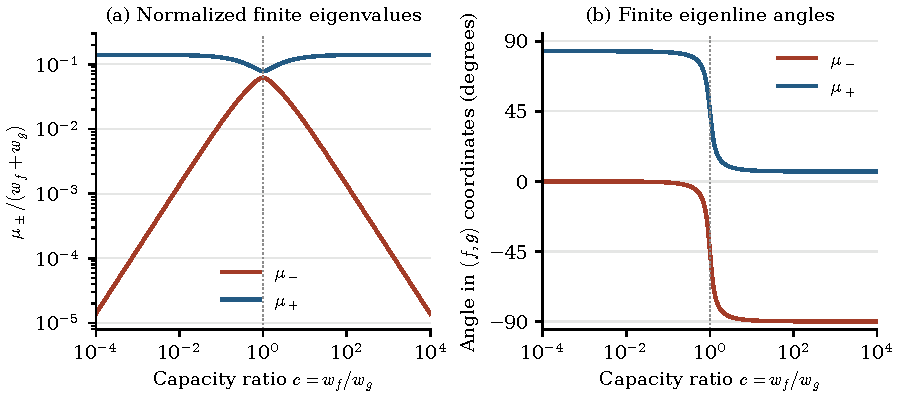
\includegraphics[width=\textwidth]{output/figures/finite_pair.pdf}
 \caption{The finite pair $(\operatorname{diag}(c,1),M)$, with quotient mass $M$.
 Left: its generalized eigenvalues divided by $1+c$.
 Right: the angles of eigenline representatives with positive
 first coordinate in the displayed $(f,g)$ basis.
 The dotted line marks equal capacities.}
 \label{fig:finite-pair}
\end{figure}

\subsection{Realized logarithmic hierarchies}

For positive functions $F(h),G(h)\to\infty$,
the admissible slice
\begin{equation}\label{eq:general-exponential-slice}
 p(h)=(a,a,a,-3a;\ b,b,b,-3b),\qquad
                  a=e^{-F(h)},\quad b=e^{-G(h)}
\end{equation}
eventually belongs to $B^\circ$.
The bounded holomorphic units and the
factor $-3$ change each logarithm by a
bounded amount. Hence
\[
 w_f\sim\frac{8\pi}{F(h)},\qquad
 w_g\sim\frac{8\pi}{G(h)}.
\]
If $F/G\to0$, the actual simple
eigenvalues satisfy
\begin{equation}\label{eq:actual-general-hierarchy}
 \lambda_+\sim\frac{9\pi}{8F(h)},\qquad
 \lambda_-\sim\frac{10\pi}{9G(h)}.
\end{equation}
Taking $F=h^{-1}$, $G=h^{-2}$ gives
the constants in \eqref{eq:separated-spectrum-intro}.
Taking $G=h^{-1}\log(1/h)$ instead gives
the orders $h$ and $h/\log(1/h)$;
taking $G=h^{-1}\log\log(1/h)$ gives
$h$ and $h/\log\log(1/h)$. These are
paths on the actual family; they are
not holomorphic arcs at the origin.
This completes the eigenline and path
consequences announced after
Theorem~\ref{thm:main}.

\subsection{Fixed cutoffs and exterior identifications}

Keep $W,M$ fixed, but choose two compact
central exteriors $C_1,C_2$ with their
central-metric closed projections and
cohomology maps. Let $\mathcal A_1,
\mathcal A_2$ be the resulting observers.
Choose a larger compact exterior $C$
containing both, and set $\zeta=\Pi_Cu$.
The class of this closed form agrees
on both smaller exteriors, so
$\mathcal A_1\zeta=\mathcal A_2\zeta$.
The first-order projection estimate gives
\begin{equation}\label{eq:fixed-cutoff-discrepancy}
 \|(\mathcal A_2-\mathcal A_1)u\|_M
       \le C\|\dd u\|_{L^2(C,g_p)}.
\end{equation}
Here the actual and central exterior
metrics are uniformly equivalent.
The constants may depend on these fixed
choices.

On $S_p$, put
$B_p=\mathcal A_2(\mathcal A_1|_{S_p})^{-1}$
and $\sigma_p=\max\Eig(E_p,M)$.
Equation \eqref{eq:fixed-cutoff-discrepancy}
and the mass and energy estimates show
that $\mathcal A_2$ is also invertible
for small $p$, and
\begin{equation}\label{eq:cutoff-relative-transport}
 \begin{aligned}
 \|B_p-I\|_M&\le C\sqrt{\sigma_p},\\
 \sqrt{E_p((B_p-I)x)}
       &\le C\sqrt{\sigma_p}\sqrt{E_p(x)}.
 \end{aligned}
\end{equation}
For the second line, use
$E_p(y)\le\sigma_pM(y)$ and
$q_p(\mathcal A_1^{-1}x)\le(1+o(1))E_p(x)$.
The first follows from the cluster bound
$q_p\le C\sigma_p\|\cdot\|^2$.
The triangle inequality in the energy
seminorm gives
\[
 (1-C\sqrt{\sigma_p})E_p
       \le B_p^*E_pB_p
       \le(1+C\sqrt{\sigma_p})E_p,
\]
after changing $C$, and the mass obeys
the analogous estimate. The observed
forms transform exactly as
$B_p^*Q_{2,p}B_p=Q_{1,p}$ and
$B_p^*N_{2,p}B_p=N_{1,p}$.
Thus both observers give the same
relative description without a
lower bound on the eigenvalue ratio.

The same conclusion holds when exterior
identifications differ by a smooth isotopy
preserving the relevant exterior, with
uniform derivative, inverse-Jacobian and
generating-vector-field bounds.
The homotopy formula reads
$F_1^*u-F_0^*u=\dd Ku+K\dd u$.
The observation of the exact term is
zero, and the other term is bounded
by $C\|\dd u\|$. Density extends the
argument to form-domain inputs.
An arbitrary shrinking cutoff or
unbounded isotopy requires another
estimate. Phase interpolations supported
in the necks leave the fixed exterior
observer unchanged.

\subsection{Coordinates, polarization and base change}

Under a finite coordinate change $x=Sx'$,
the data transform as
\[
 E'=S^*ES,\qquad M'=S^*MS,\qquad
                       \mathcal A'=S^{-1}\mathcal A.
\]
Generalized eigenvalues and intrinsic
relative inequalities are unchanged,
and subspaces are transported by $S$.
No Euclidean condition-number bound on
$S$ is needed. An integral marking
change must preserve the specified
lattice; this observation does not
supply a lattice from spectral data.

A permitted analytic node-coordinate
change has the form
$\tau'_i=u_i(p)\tau_{\pi(i)}$,
with holomorphic units bounded above
and away from zero. Transport the
link generators by their signs and
permutation. Then
\[
 |\log|\tau'_i||=|\log|\tau_{\pi(i)}||+O(1),
\]
so $E'_p$ and $E_p$ differ relatively
by $O(L_{\min}^{-1})$. This follows
term by term from the reciprocal
lengths and the nonnegative period
squares. The geometric mass transforms
by congruence.
Lemma~\ref{lem:relative-subspace-transport}
and \eqref{eq:uniform-conifold-gap}
give an $O(L_{\min}^{-1})$ change of
the transported finite eigenlines.

Polarization is genuine geometric
input. Scaling the Kähler class by
a fixed $c>0$ scales the Ricci-flat
metric by $c$. In real dimension six
the two-form squared $L^2$ norm scales
by $c$, whereas its $\dd$-energy
scales by one. The eigenvalues
therefore scale by $c^{-1}$.

For a holomorphic base map with
$\tau_i(s)=a_is^{\nu_i}+O(s^{\nu_i+1})$,
$a_i\ne0$ and $\nu_i>0$,
\begin{equation}\label{eq:holomorphic-arc-capacity}
 \frac{2\pi}{|\log|\tau_i(s)||}
       \sim\frac{2\pi}{\nu_i|\log|s||}.
\end{equation}
All capacities have one logarithmic
order. A ramification $s=v^m$ multiplies
every $\nu_i$ by $m$ and divides the
leading coefficients expressed in
$|\log|v||$ by $m$. This reparametrizes
fibres; it does not preserve a
coefficient in a fixed parameter.
For an admissible monomial map
$\tau_i(z)=u_i(z)\prod_jz_j^{a_{ij}}$,
the corresponding length is
$\sum_ja_{ij}|\log|z_j||+O(1)$.
Such a map must factor through the
actual relation base and smooth
the selected nodes. Eight arbitrarily
prescribed monomials need not do so.

\section{Attachment maps, monodromy and the spectral hierarchy}
\label{sec:topology-comparison}

\subsection{Relations among vanishing cycles}

Let $Y$ be the small resolution, $U$ the common exterior,
$C_i$ the exceptional curves, and $\delta_i$ the oriented
vanishing spheres. The integral Thom and Mayer--Vietoris
calculation in \cite[Section~3.3, proposition on restriction
and spectral coefficient]{wuebben-hodge} gives
\begin{equation}\label{eq:integral-conifold-sequence}
 \begin{aligned}
 0\longrightarrow H^2(X_p;\ZZ)
 &\longrightarrow H^2(Y;\ZZ)
 \xrightarrow{\ r\ }\ZZ^8
 \xrightarrow{\ \partial\ }H^3(X_p;\ZZ)\\
 &\longrightarrow H^3(U;\ZZ)\longrightarrow0,
 \end{aligned}
\end{equation}
where $r(D)_i=D\cdot C_i$ and
$\partial e_i=\operatorname{PD}_L(\delta_i)$.
The latter class is defined by the oriented Thom
construction, including any torsion in its global image.

Over $\QQ$, put
$Q_{\mathrm{lost}}=H^2(Y;\QQ)/\im H^2(X_p;\QQ)$
and $V_{\mathrm{van}}=\im\partial$. Then
\begin{equation}\label{eq:rational-conifold-sequence}
 0\longrightarrow Q_{\mathrm{lost}}
 \xrightarrow{\ r\ }\QQ^8
 \xrightarrow{\ \partial\ }V_{\mathrm{van}}
 \longrightarrow0.
\end{equation}
Their dimensions are two and six, respectively.
In our quotient basis the columns of $r$ are
$(1,1,1,1;0,0,0,0)$ and $(0,0,0,0;1,1,1,1)$.
Thus the lost degree-two cohomology quotient is the space of
relations among the cohomological vanishing cycles,
and its composite to $V_{\mathrm{van}}$ is zero.
The exceptional-curve map $s:\QQ^8\to H_2(Y;\QQ)$,
$s(e_i)=[C_i]$, is dual to $r$.
Its six-dimensional relation space $\ker s$ is
a different space, paired with the period
coordinates of Section~\ref{sec:geometry}.

Lee--Lin--Wang realize
\eqref{eq:rational-conifold-sequence} as the
rational weight-two basic exact sequence of a
semistable model \cite[Theorem~1.14]{lee-lin-wang};
their Proposition~3.16 treats vanishing-period
coordinates. These are classical deformation
and Hodge-theoretic inputs. Rational exactness
does not by itself establish integral saturation
or recover an unknown attaching map.

\subsection{The nearby-cycle sequence}

For a specified proper one-parameter
ordinary-double-point smoothing $f$ with
smooth total space, the unshifted nearby-
and vanishing-cycle triangle is
\[
 i^*\QQ\longrightarrow R\psi_f\QQ
 \longrightarrow R\phi_f\QQ
 \longrightarrow i^*\QQ[1].
\]
The Milnor fibres of the threefold nodes
give the specialization segment
\begin{equation}\label{eq:nearby-cycle-sequence}
 \begin{aligned}
 0\longrightarrow H^3(X_0;\QQ)
 &\longrightarrow H^3(X_t;\QQ)
 \xrightarrow{\ \mathrm{can}\ }\QQ^8\\
 &\longrightarrow H^4(X_0;\QQ)
 \longrightarrow H^4(X_t;\QQ)\longrightarrow0.
 \end{aligned}
\end{equation}
The map $\mathrm{can}$ evaluates on vanishing
spheres. Its image annihilates the relations
in \eqref{eq:rational-conifold-sequence}.
The map $\partial$ there is its
Poincaré--excision dual, with the chosen
orientation convention; it is not the arrow
from $\QQ^8$ to $H^4(X_0;\QQ)$ in
\eqref{eq:nearby-cycle-sequence}.
For the triangles, stalks and canonical/variation
identities see \cite[Section~3]{massey}, and
for the conifold specialization see
\cite[Section~1]{lee-lin-wang}.
After ramified base change the total space
need not be smooth; one must use nearby-cycle
base change or a semistable model instead of
applying the smooth-total-space local argument
without its hypothesis.

\subsection{What monodromy does not determine}

Picard--Lefschetz gives
$N_i\gamma=\pm\langle\gamma,\delta_i\rangle\delta_i$.
The vanishing spheres are disjoint, so
$N_iN_j=0$. For an all-node loop with
positive winding numbers $\nu_i$,
\begin{equation}\label{eq:all-node-monodromy}
 T=I+N,\qquad N=\sum_i\nu_iN_i,\qquad N^2=0
\end{equation}
as in \cite[Section~3.3, equation (3.4)]{lee-lin-wang}.
The monodromy image is abelian; no assertion
that the fundamental group of the
discriminant complement is abelian is needed.

The weight filtration centred at three is
\begin{equation}\label{eq:monodromy-weight-filtration}
 0=W_1\subset W_2=\im N
       \subset W_3=\ker N\subset W_4=H^3.
\end{equation}
Here $\dim W_2=6$. These rational subspaces
are independent of the positive $\nu_i$.
In a symplectic basis let $B$ have columns
$\delta_i$ and let $J$ be the intersection
matrix. Then $N=\pm BDB^{\mathsf T}J$,
$D=\operatorname{diag}(\nu_i)>0$.
The matrix $BDB^{\mathsf T}$ has the
same rank and image as $B$, so
$\im N=\im B$ and
$\ker N=(\im B)^{\perp_J}$.
Integral image indices can change under
ramification. The characterization of the
weight filtration is
\cite[Section~6, Lemma~(6.4)]{schmid};
the identification of $V_{\mathrm{van}}$
with $W_2$ is
\cite[Lemma~1.12]{lee-lin-wang}.

The two admissible paths
\[
 (a,b)=(e^{-h^{-1}},e^{-h^{-2}})
 \quad\hbox{and}\quad
 (a,b)=(e^{-h^{-1}},e^{-h^{-3}})
\]
have the same marked central attachment
sequence and local monodromy representation.
Choose the same reference all-node loop;
its operator and weight filtration are
then the same. Nevertheless
\eqref{eq:actual-general-hierarchy} gives
the actual spectral orders $(h,h^2)$ and
$(h,h^3)$. The stated topology and monodromy
data therefore do not determine the
capacity hierarchy.

An interval path has no distinguished loop,
and a nonanalytic path does not define an
ordinary holomorphic-disc nearby-cycle
functor. We make no assertion that the
full limiting mixed Hodge structures or
period asymptotics agree on these paths.
The limiting Hodge filtration contains
further information; its coordinate
dependence by $\exp(cN)$ is recorded
before \cite[Theorem~(6.16)]{schmid}.

\subsection{Comparison with adiabatic spectral sequences}

For a fixed compact fibration,
Mazzeo--Melrose identify the adiabatic
Hodge problem with the Leray spectral
sequence \cite[Theorems~(7), (15) and
Corollary~(18)]{mazzeo-melrose}.
For a fixed smooth Riemannian foliation
on a closed manifold, Álvarez
López--Kordyukov study
$g_h=h^{-2}g_\perp+g_F$.
The transverse-degree filtration gives
\[
 \dd_h=\dd_{0,1}+h\dd_{1,0}+h^2\dd_{2,-1}.
\]
Their Theorem~A counts eigenvalues,
including zeros, of order $O(h^{2k})$
by the degreewise dimension of the
$k$-th page for $k\ge2$; at $k=1$
it uses the Hausdorff quotient of
the first page \cite{alvarez-kordyukov}.
The corrected Theorem~B gives only
weak subsequential convergence at
$k=1$ in its stated setting, with
strong convergence for $k\ge2$
under its energy hypotheses.

Those results include a filtered
differential complex and its page
differentials. The successive kernels
in Theorem~\ref{thm:fixed-map-hierarchy}
come instead from the fixed restriction
rows of a finite energy form.
We have not constructed page differentials
or a compatible de Rham Laplacian in
every degree. The conifold smoothing
also changes topology, unlike the
fixed-foliation adiabatic metric.
Thus neither the capacity groups nor
the relation space in
\eqref{eq:rational-conifold-sequence}
are identified with those pages.

\begin{thebibliography}{LLW18}

\bibitem[ARS18]{ars-cusps}
P.~Albin, F.~Rochon and D.~Sher,
\emph{Analytic torsion and R-torsion of Witt representations on manifolds
with cusps},
Duke Math. J. \textbf{167} (2018), 1883--1950.
\href{https://doi.org/10.1215/00127094-2018-0009}
{doi:10.1215/00127094-2018-0009}.
Locators refer to
\href{https://arxiv.org/abs/1411.1105v3}{arXiv:1411.1105v3}.

\bibitem[AK00]{alvarez-kordyukov}
J.~A.~Álvarez López and Y.~A.~Kordyukov,
\emph{Adiabatic limits and spectral sequences for Riemannian foliations},
Geom. Funct. Anal. \textbf{10} (2000), 977--1027.
The corrected statements and locators used here are in
\href{https://arxiv.org/abs/math/9902147v2}{arXiv:math/9902147v2},
including the 2025 corrigendum.

\bibitem[AT15]{anne-takahashi}
C.~Anné and J.~Takahashi,
\emph{Partial collapsing and the spectrum of the Hodge--de Rham operator},
Anal. PDE \textbf{8} (2015), no.~5, 1025--1050.
\href{https://doi.org/10.2140/apde.2015.8.1025}
{doi:10.2140/apde.2015.8.1025}.

\bibitem[Ben26]{benabida}
A.~O.~Benabida,
\emph{Asymptotics for resolutions and smoothings of Calabi--Yau conifolds},
Comm. Math. Phys. \textbf{407} (2026), article~71.
\href{https://doi.org/10.1007/s00220-026-05578-5}
{doi:10.1007/s00220-026-05578-5}.
Locators refer to
\href{https://arxiv.org/abs/2503.16702v3}{arXiv:2503.16702v3}.

\bibitem[Bur90]{burger}
M.~Burger,
\emph{Small eigenvalues of Riemann surfaces and graphs},
Math. Z. \textbf{205} (1990), 395--420.

\bibitem[CH13]{conlon-hein}
R.~J.~Conlon and H.-J.~Hein,
\emph{Asymptotically conical Calabi--Yau manifolds, I},
Duke Math. J. \textbf{162} (2013), no.~15, 2855--2902.
\href{https://doi.org/10.1215/00127094-2382452}
{doi:10.1215/00127094-2382452}.
Locators refer to
\href{https://arxiv.org/abs/1205.6347v2}{arXiv:1205.6347v2}.

\bibitem[Fre05]{frey}
C.~Frey,
\emph{On Non-local Boundary Value Problems for Elliptic Operators},
dissertation, Universität zu Köln, 2005.
\href{https://kups.ub.uni-koeln.de/1512/1/dissertation_frey.pdf}
{Institutional text}.

\bibitem[Fri26]{friedman-unobstructed}
R.~Friedman,
\emph{Unobstructed deformations for singular Calabi--Yau varieties},
preprint, February~13, 2026.
\href{https://arxiv.org/abs/2506.09857v3}{arXiv:2506.09857v3}.

\bibitem[HHM04]{hausel-hunsicker-mazzeo}
T.~Hausel, E.~Hunsicker and R.~Mazzeo,
\emph{Hodge cohomology of gravitational instantons},
Duke Math. J. \textbf{122} (2004), no.~3, 485--548.
\href{https://doi.org/10.1215/S0012-7094-04-12233-X}
{doi:10.1215/S0012-7094-04-12233-X}.

\bibitem[HS17]{hein-sun}
H.-J.~Hein and S.~Sun,
\emph{Calabi--Yau manifolds with isolated conical singularities},
Publ. Math. Inst. Hautes Études Sci. \textbf{126} (2017), 73--130.
\href{https://doi.org/10.1007/s10240-017-0092-1}
{doi:10.1007/s10240-017-0092-1}.

\bibitem[Kle05]{kleiman-picard}
S.~L.~Kleiman,
\emph{The Picard scheme},
in \emph{Fundamental Algebraic Geometry: Grothendieck's FGA Explained},
Mathematical Surveys and Monographs, vol.~123,
American Mathematical Society, Providence, RI, 2005, 235--321.
Locators refer to
\href{https://arxiv.org/abs/math/0504020v1}{arXiv:math/0504020v1}.

\bibitem[LLW18]{lee-lin-wang}
Y.-P.~Lee, H.-W.~Lin and C.-L.~Wang,
\emph{Towards $A+B$ theory in conifold transitions for Calabi--Yau
threefolds},
J. Differential Geom. \textbf{110} (2018), 495--541.
\href{https://doi.org/10.4310/jdg/1542423628}
{doi:10.4310/jdg/1542423628}.
Locators refer to
\href{https://arxiv.org/abs/1502.03277v3}{arXiv:1502.03277v3}.

\bibitem[Mas14]{massey}
D.~B.~Massey,
\emph{Milnor fibers and links of local complete intersections},
Internat. J. Math. \textbf{25} (2014), article~1450110.
\href{https://doi.org/10.1142/S0129167X14501109}
{doi:10.1142/S0129167X14501109}.
Locators refer to
\href{https://arxiv.org/abs/1402.5276v1}{arXiv:1402.5276v1}.

\bibitem[MM90]{mazzeo-melrose}
R.~Mazzeo and R.~Melrose,
\emph{The adiabatic limit, Hodge cohomology and Leray's spectral
sequence for a fibration},
J. Differential Geom. \textbf{31} (1990), 185--213.

\bibitem[Pac13]{pacini}
T.~Pacini,
\emph{Desingularizing isolated conical singularities: uniform estimates
via weighted Sobolev spaces},
Comm. Anal. Geom. \textbf{21} (2013), no.~1, 105--170.
\href{https://doi.org/10.4310/CAG.2013.v21.n1.a3}
{doi:10.4310/CAG.2013.v21.n1.a3}.
Locators refer to
\href{https://arxiv.org/abs/1005.3511v3}{arXiv:1005.3511v3}.

\bibitem[RT09]{rollenske-thomas}
S.~Rollenske and R.~Thomas,
\emph{Smoothing nodal Calabi--Yau $n$-folds},
J. Topol. \textbf{2} (2009), no.~2, 405--421.
\href{https://doi.org/10.1112/jtopol/jtp016}{doi:10.1112/jtopol/jtp016}.
Locators refer to the corrected
\href{https://arxiv.org/abs/0810.0141v3}{arXiv:0810.0141v3}.

\bibitem[Sch73]{schmid}
W.~Schmid,
\emph{Variation of Hodge structure: the singularities of the period mapping},
Invent. Math. \textbf{22} (1973), 211--319.
\href{https://doi.org/10.1007/BF01389674}
{doi:10.1007/BF01389674}.

\bibitem[Sta]{stacks}
The Stacks Project Authors, \emph{The Stacks Project},
\href{https://stacks.math.columbia.edu/tag/055S}{Tag~055S}.

\bibitem[W26a]{wuebben-hodge}
B.~J.~Wuebben,
\emph{Integral topology and small eigenvalues in Calabi--Yau conifold
transitions}, preprint, November~9, 2026.
\href{https://doi.org/10.5281/zenodo.24096887}
{doi:10.5281/zenodo.24096887}.

\bibitem[W26b]{wuebben-chambers}
B.~J.~Wuebben,
\emph{Nonsimplicial local stability chambers of toric tangent bundles},
preprint, October~29, 2026.
\href{https://doi.org/10.5281/zenodo.23774770}
{doi:10.5281/zenodo.23774770}.

\end{thebibliography}

\end{document}
